YOLO significa \textit{You Only Look Onc}e\  \url{https://pjreddie.com/darknet/yolo/}. Se le puso ese nombre debido a que la red neuronal solo se aplica una vez a la imagen completa, lo que permite una detección rápida y precisa de objetos. Una de las ventajas clave de YOLO es que puede detectar múltiples objetos en una sola imagen, prediciendo las etiquetas de clase y las ubicaciones de los objetos al mismo tiempo. La red neuronal divide la imagen en regiones, predice cajas delimitadoras o \textit{bounding boxes} y probabilidades para cada una de ellas, y filtra las cajas delimitadoras con una técnica llamada supresión no máxima para eliminar aquellas con baja confianza o superpuestas con otras de mayor confianza \cite{yolo1}.\\

El origen de YOLO se remonta al año 2015, fue desarrollado por Joseph Redmon, Santosh Divvala, Ross Girshick y Ali Farhadi mientras trabajaban en la Universidad de Washington. La primera versión de YOLO se presentó en un artículo titulado "\textit{You Only Look Once: Unified, Real-Time Object Detection}" en la conferencia de visión por ordenador CVPR (Computer Vision and Pattern Recognition) en 2016. \\

El éxito de YOLO se debió en gran parte a su capacidad para detectar objetos en tiempo real, con una velocidad de procesamiento mucho más rápida que otros algoritmos. Además, su precisión en la detección de objetos en imágenes fue muy alta en comparación en comparación con otros.\\

En 2016, Joseph Redmon fundó una empresa llamada "YOLO: You Only Look Once Inc." para desarrollar la tecnología de detección de objetos YOLO en un producto comercial. Sin embargo, en 2018, Redmon anunció que se retiraba de la investigación en inteligencia artificial debido a sus preocupaciones éticas sobre el uso de la tecnología de IA en aplicaciones militares.\\

A partir de entonces, la investigación y el desarrollo de YOLO fueron continuados por otros investigadores. Actualmente, hay cuatro versiones oficiales de YOLO: YOLOv1, YOLOv2, YOLOv3 y YOLOv4, donde cada versión ha mejorado en términos de precisión y velocidad de procesamiento, y ha incorporado nuevas técnicas de detección de objetos, como la eliminación de falsos positivos \cite{yolo2}.\\

En concreto, nosotros vamos a utilizar YOLO versión 3, la cual utiliza 53 capas convolucionales sucesivas. Seleccionamos esta versión ya que, debido al auge de estas tecnologías, quizás sea la versión con mayor documentación y ejemplos de los cuales aprender.\\

Lo normal cuando un particular se plantea desarrollar un proyecto de este tipo es trabajar a través de Google Colab o mediante sus propios recursos locales. Google Colab es una herramienta en línea que permite escribir, ejecutar y compartir código Python en un entorno de notebook en la nube con acceso a recursos \textit{hardware} de alta calidad y herramientas de desarrollo preinstaladas. Sin embargo, a pesar de que nuestros ordenadores no están especialmente pensados para trabajar con IA, decidimos utilizarlos frente a la plataforma de Google. Utilizando nuestros propios recursos optamos por premiar la sencillez y facilidad de trabajo frente a la alternativa de poseer un mejor \textit{hardware} online.\\

Dado que estamos hablando de software abierto, existen numerosas versiones de cada YOLO hechas por particulares. No obstante, la tercera versión oficial de YOLO se nutre de tres ficheros de configuración, el fichero de clases, el fichero que contiene la configuración de YOLO y el fichero que contiene los pesos resultados del entrenamiento del modelo.\\

Por defecto, viene pre-entrenado con el conjunto de datos COCO (\textit{Common Objects in Context}), que es un conjunto de datos de detección de objetos, que contiene más de 330.000 imágenes etiquetadas con más de 2,5 millones de instancias de objetos de 80 categorías diferentes, incluyendo personas, animales, vehículos, muebles y objetos de la vida cotidiana. Dicho pre-entrenamiento puede resultar muy útil para numerosas aplicaciones. Sin embargo, dado que nosotros queremos desplegar un sistema dedicado únicamente a la detección de señales de tráfico, trabajaremos con unos pesos especiales destinados a dicha operación.\\

El entrenamiento de algoritmos de detección de objetos puede ser muy costoso computacionalmente. El proceso de entrenamiento puede llevar varias horas, días o incluso semanas, dependiendo del tamaño del conjunto de datos y los recursos \textit{hardware} disponibles. Por ello, decidimos partir de pesos ya pre-entrenados en detección de señales.\\

Los pesos utilizados están preparados para detectar cuatro grupos de señales diferentes:\\
\begin{itemize}
\item Prohibición: señales circulares con fondo blanco y borde rojo, como puede ser una prohibición de superar una determinada velocidad o la prohibición de entrada de un vehículo en vía.
\item Peligro: señales triangulares con fondo blanco y borde rojo, como puede ser la señal de advertencia de una curva peligrosa o peligro de desprendimientos.
\item Obligación: señales circulares azules, como puede ser la obligación de superar determinada velocidad u obligación de realizar un giro.
\item Otros: resto de señales de tráfico.
\end{itemize}

Bajo estas premisas, mediante nuestra infraestructura de red 4G podemos poner en marcha el vehículo Amazon DeepRacer que tenemos en la figura \ref{deepracer}, así podremos manejar el vehículo y acceder al contenido de su cámara.\\

\begin{figure}[H]
    \centering
 	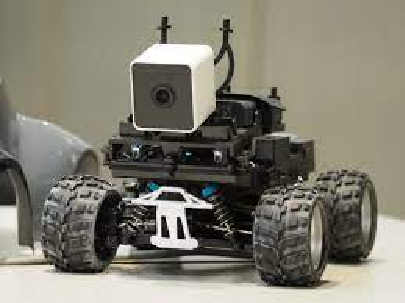
\includegraphics[width=0.6\textwidth]{Imagenes/IA/deepracer.pdf}
    \caption{Vehículo Amazon DeepRacer utilizado}
    \label{deepracer}
\end{figure}

Gracias a que nuestra escuela, ETSIT de la Universidad de Valladolid, poseía un pequeño circuito para trabajar con el vehículo, lo montamos y dispusimos varias señales de tráfico a lo largo de la maqueta. Así, pudimos probar el rendimiento de nuestro algoritmo de detección y los pesos de entrenamiento que posee. Tal y como podemos observar en las figuras \ref{deteccion1} y \ref{deteccion2}, logramos la detección de las señales a lo largo de la maqueta, a pesar de la calidad del vídeo y de que las señales miniatura no sean exactamente igual a las reales. \\

\begin{figure}[H]
    \centering
 	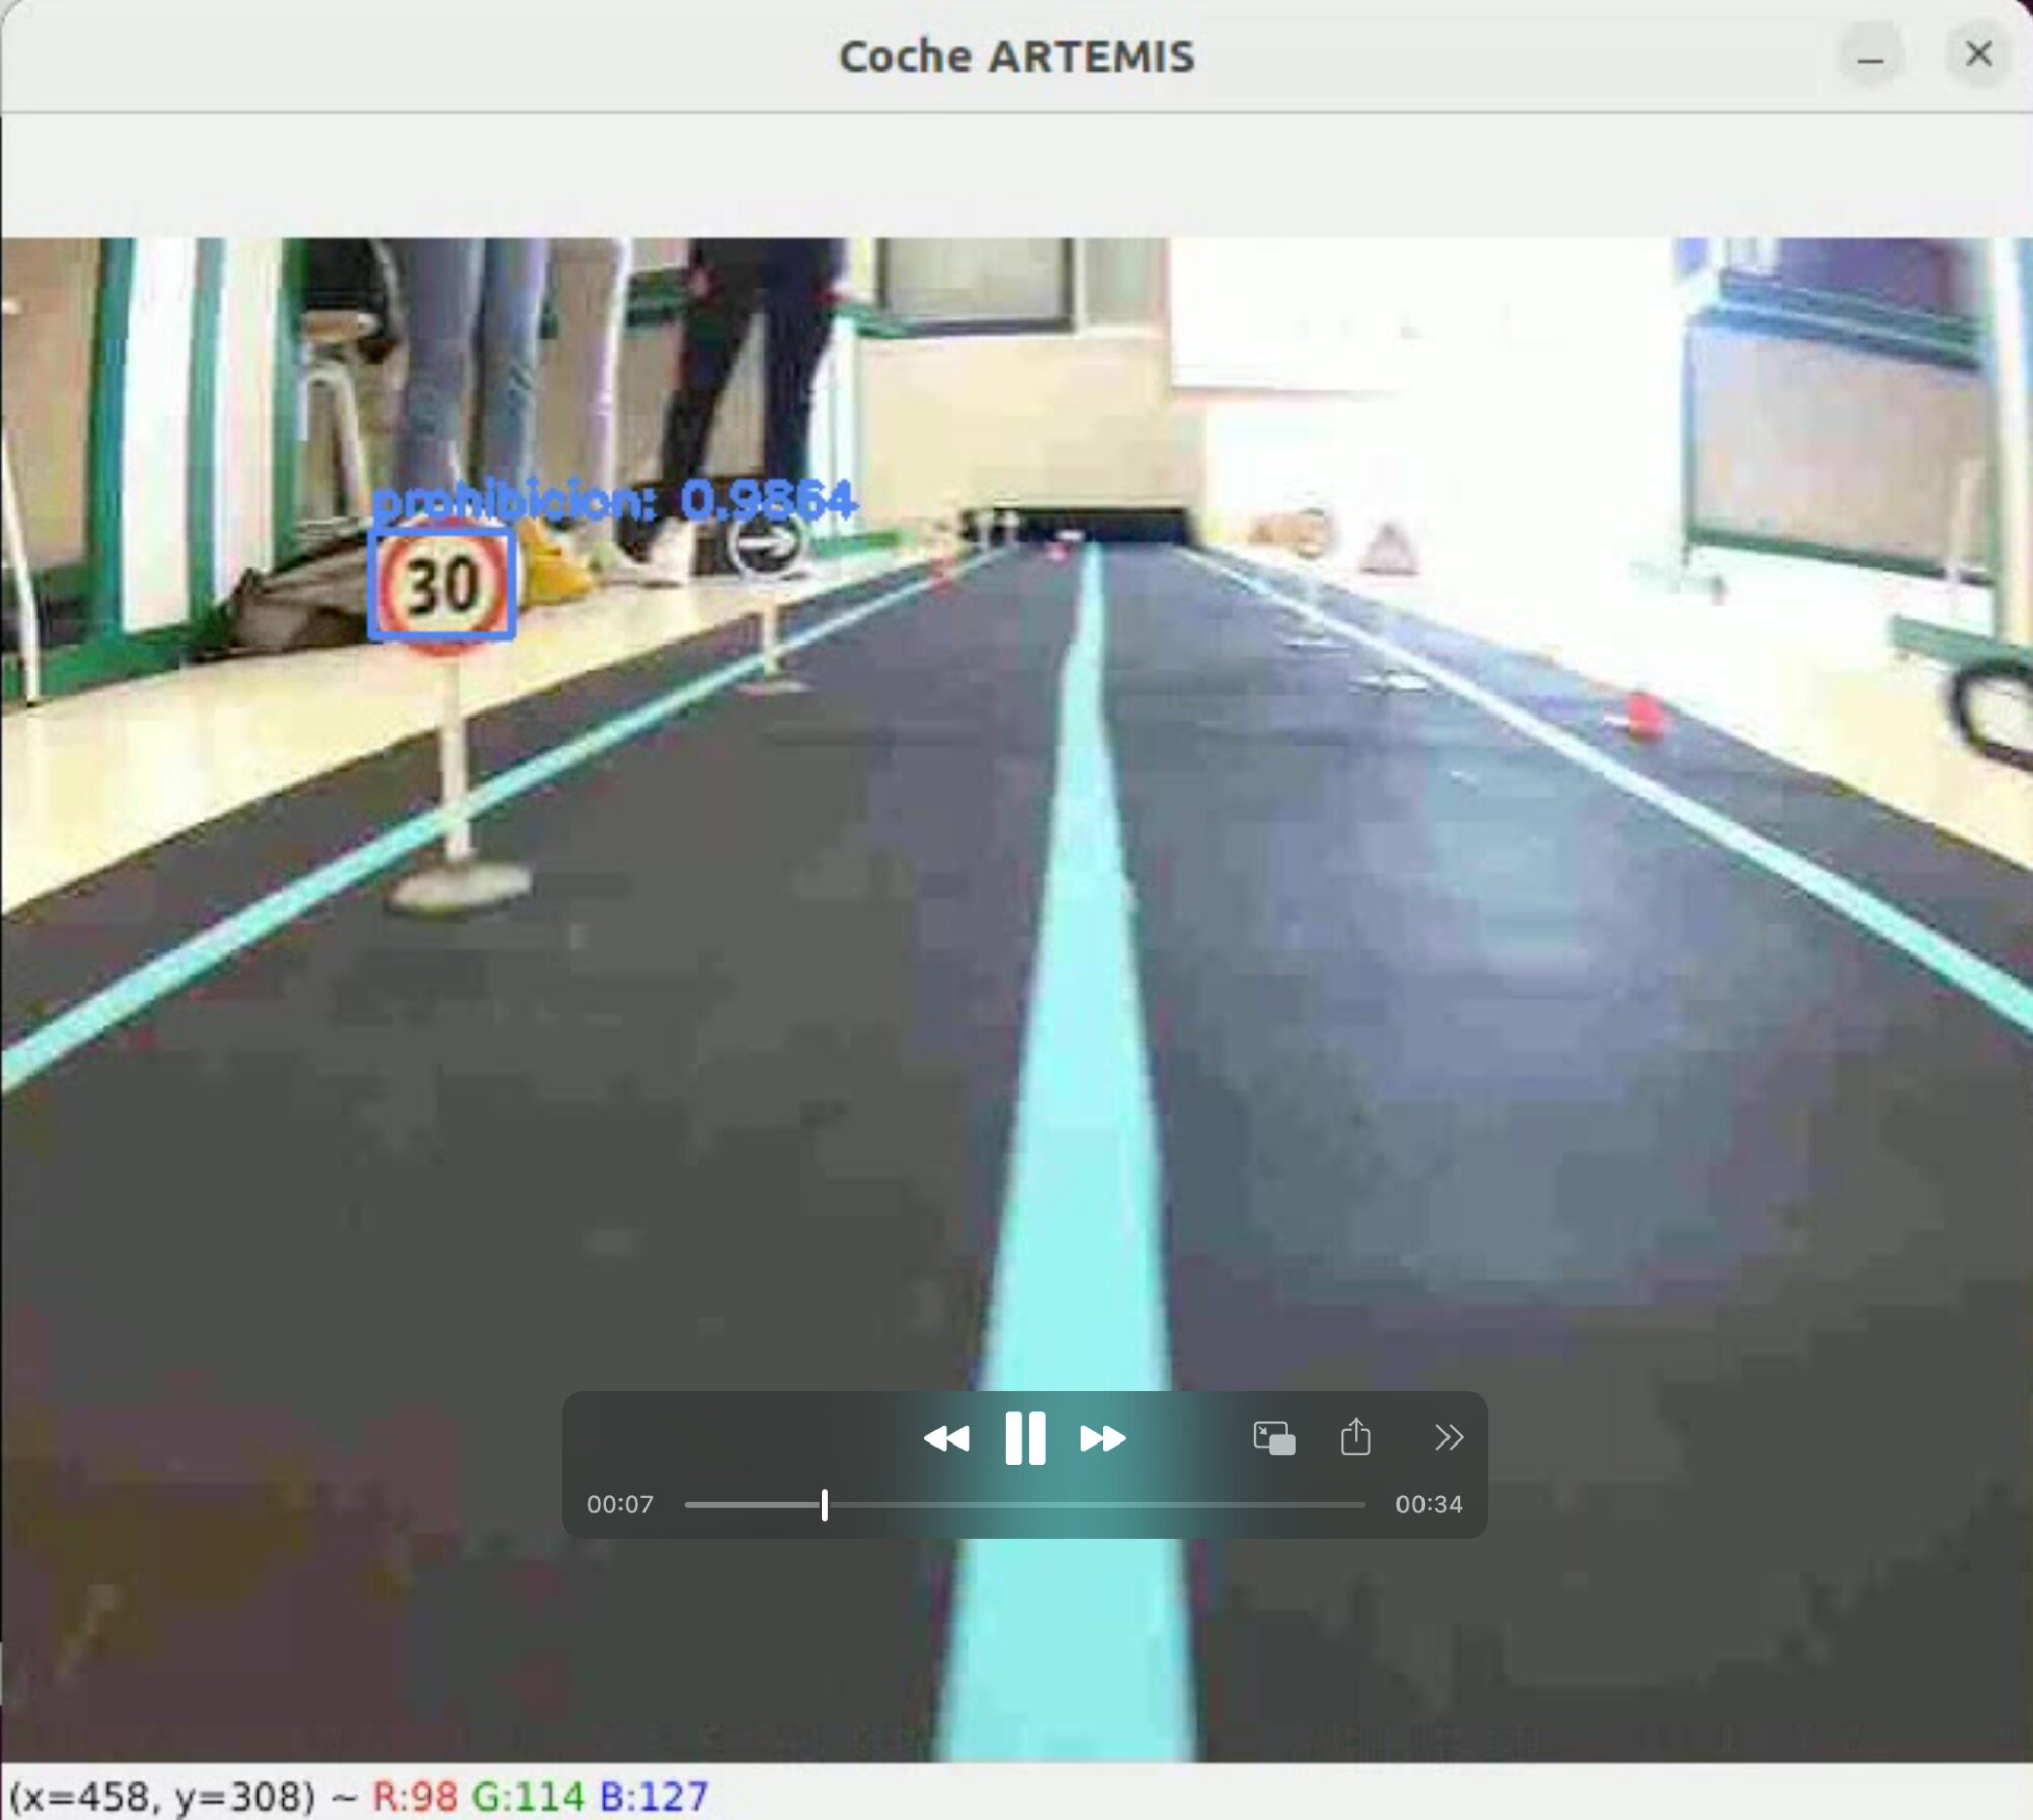
\includegraphics[width=0.6\textwidth]{Imagenes/IA/deteccion1.pdf}
    \caption{Primer ejemplo de detección de señales miniatura en vídeo en circuito}
    \label{deteccion1}
\end{figure}

\begin{figure}[H]
    \centering
 	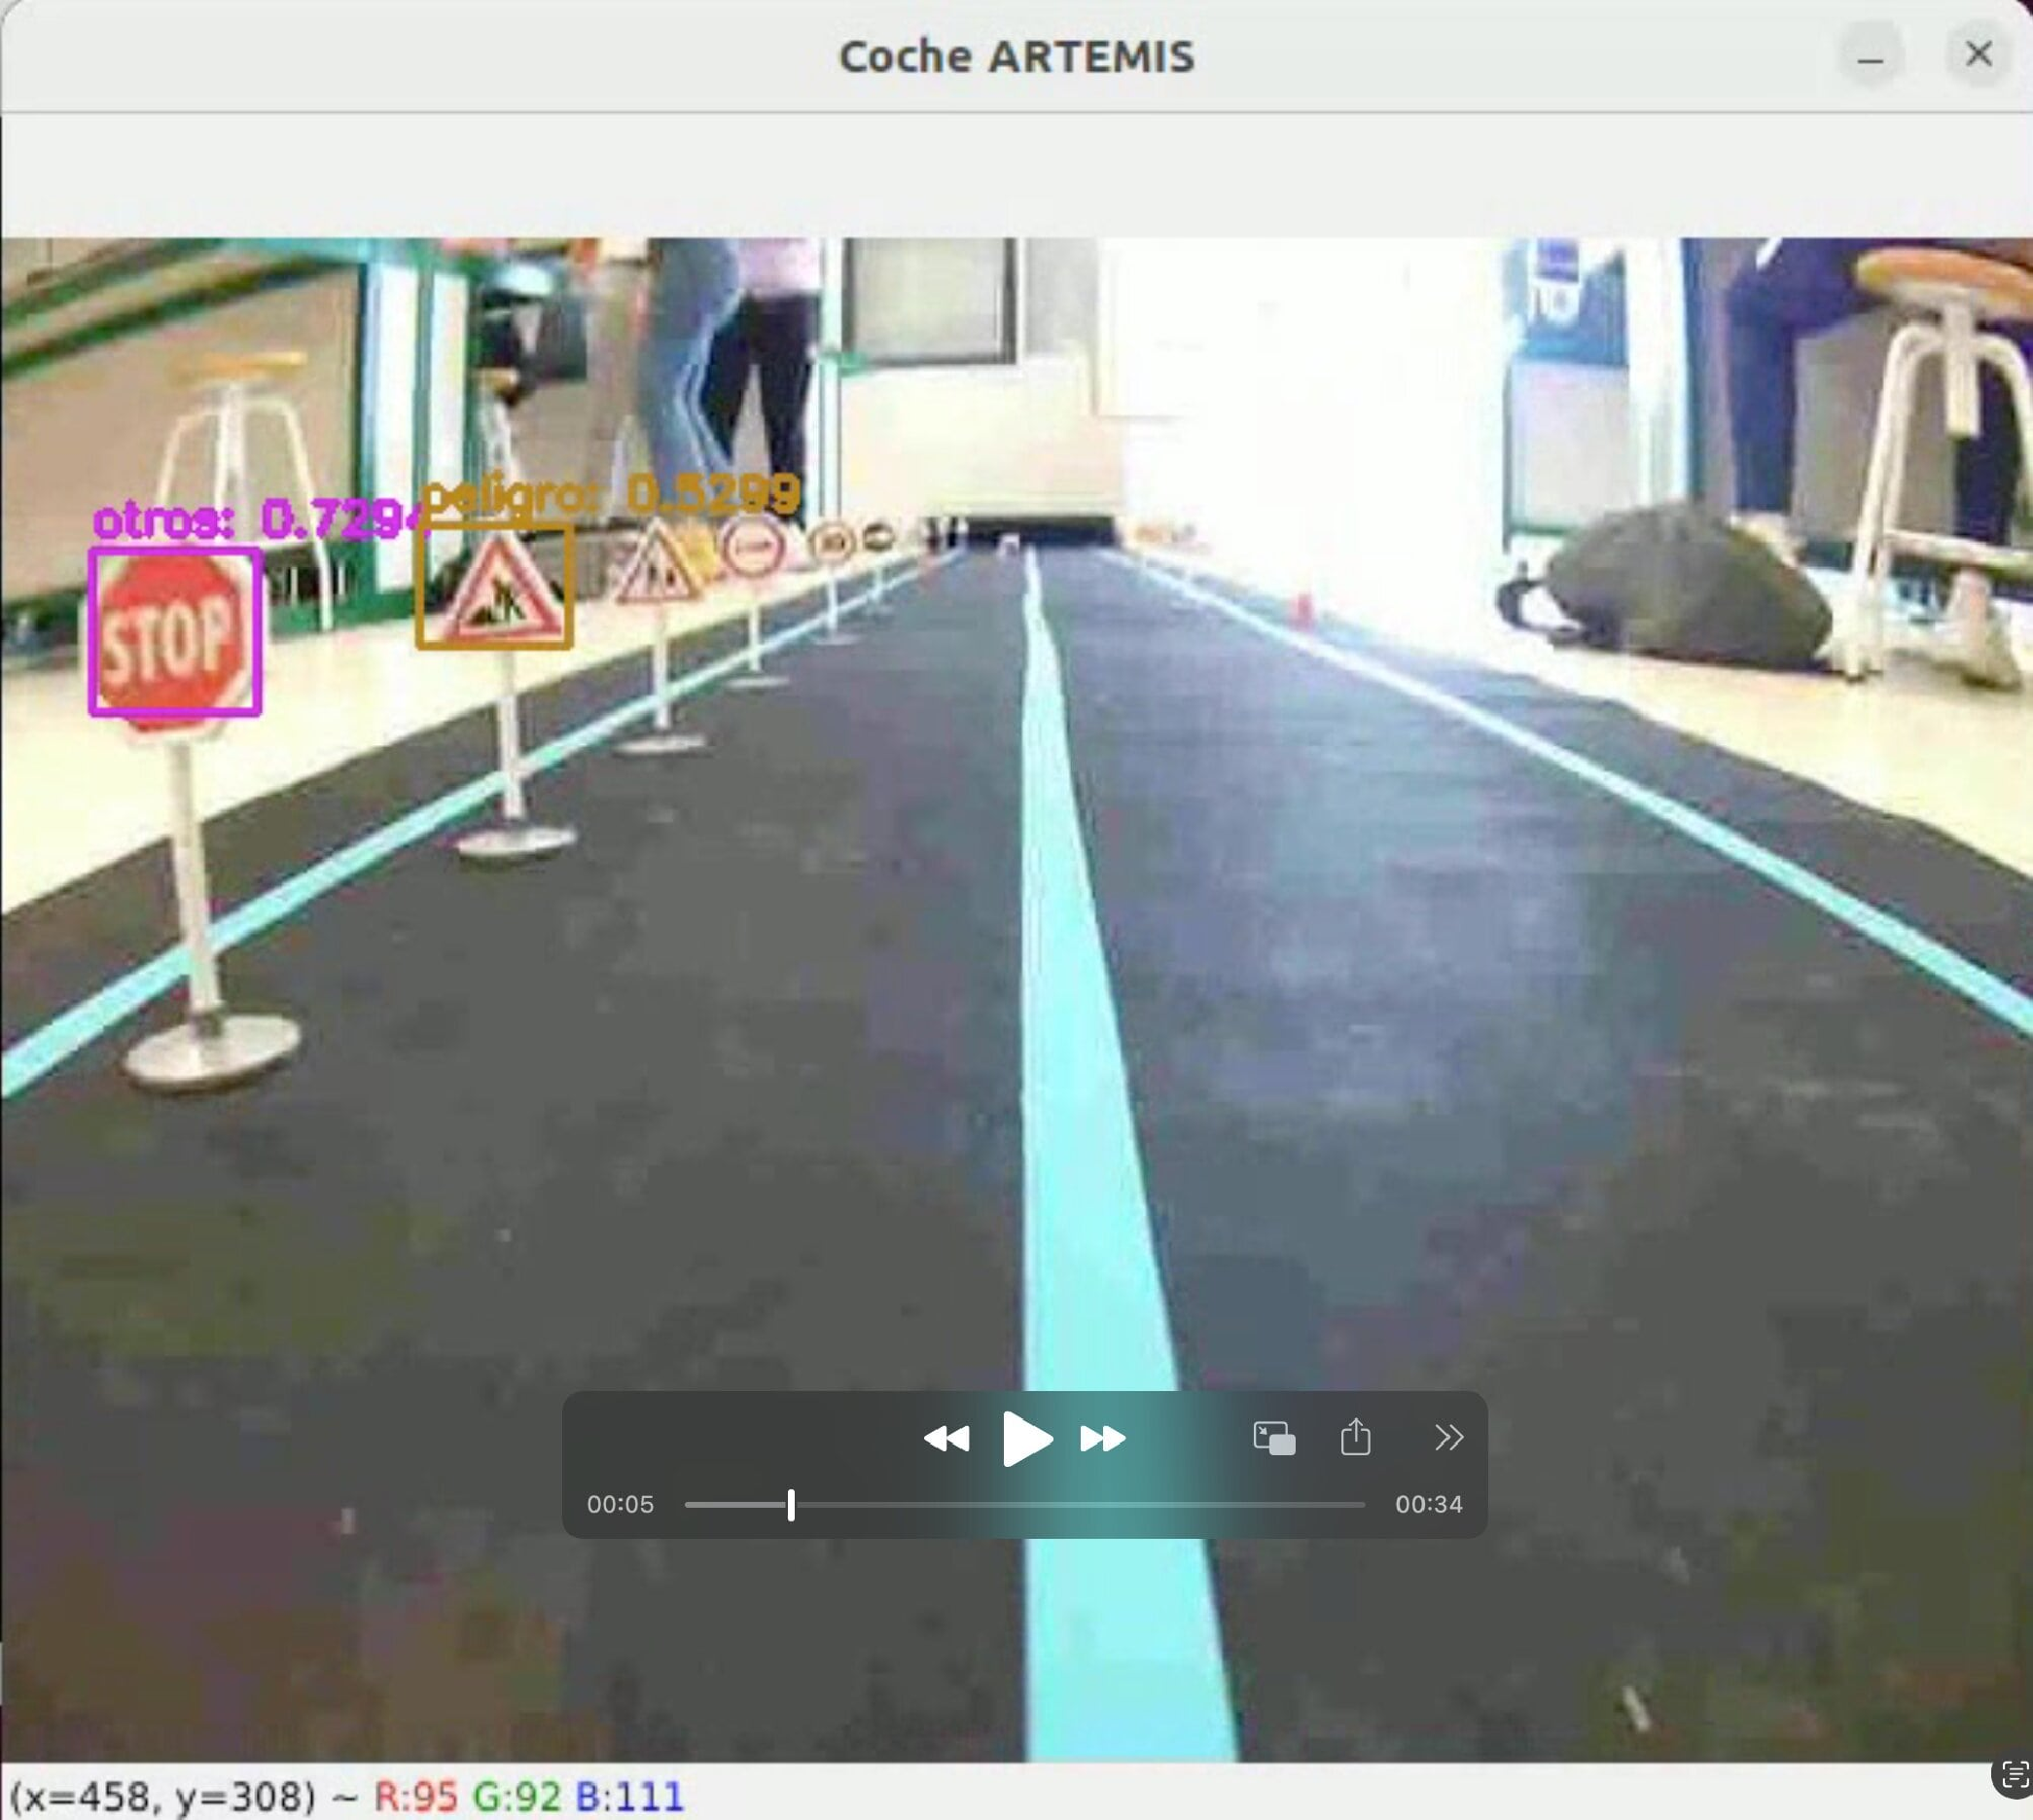
\includegraphics[width=0.6\textwidth]{Imagenes/IA/deteccion2.pdf}
    \caption{Segundo ejemplo de detección de señales miniatura en vídeo en circuito}
    \label{deteccion2}
\end{figure}

De igual forma, podemos probar con imágenes de una vía normal, podemos visualizar el procesado de nuestro algoritmo en la figura \ref{deteccion3}\\

\begin{figure}[H]
    \centering
 	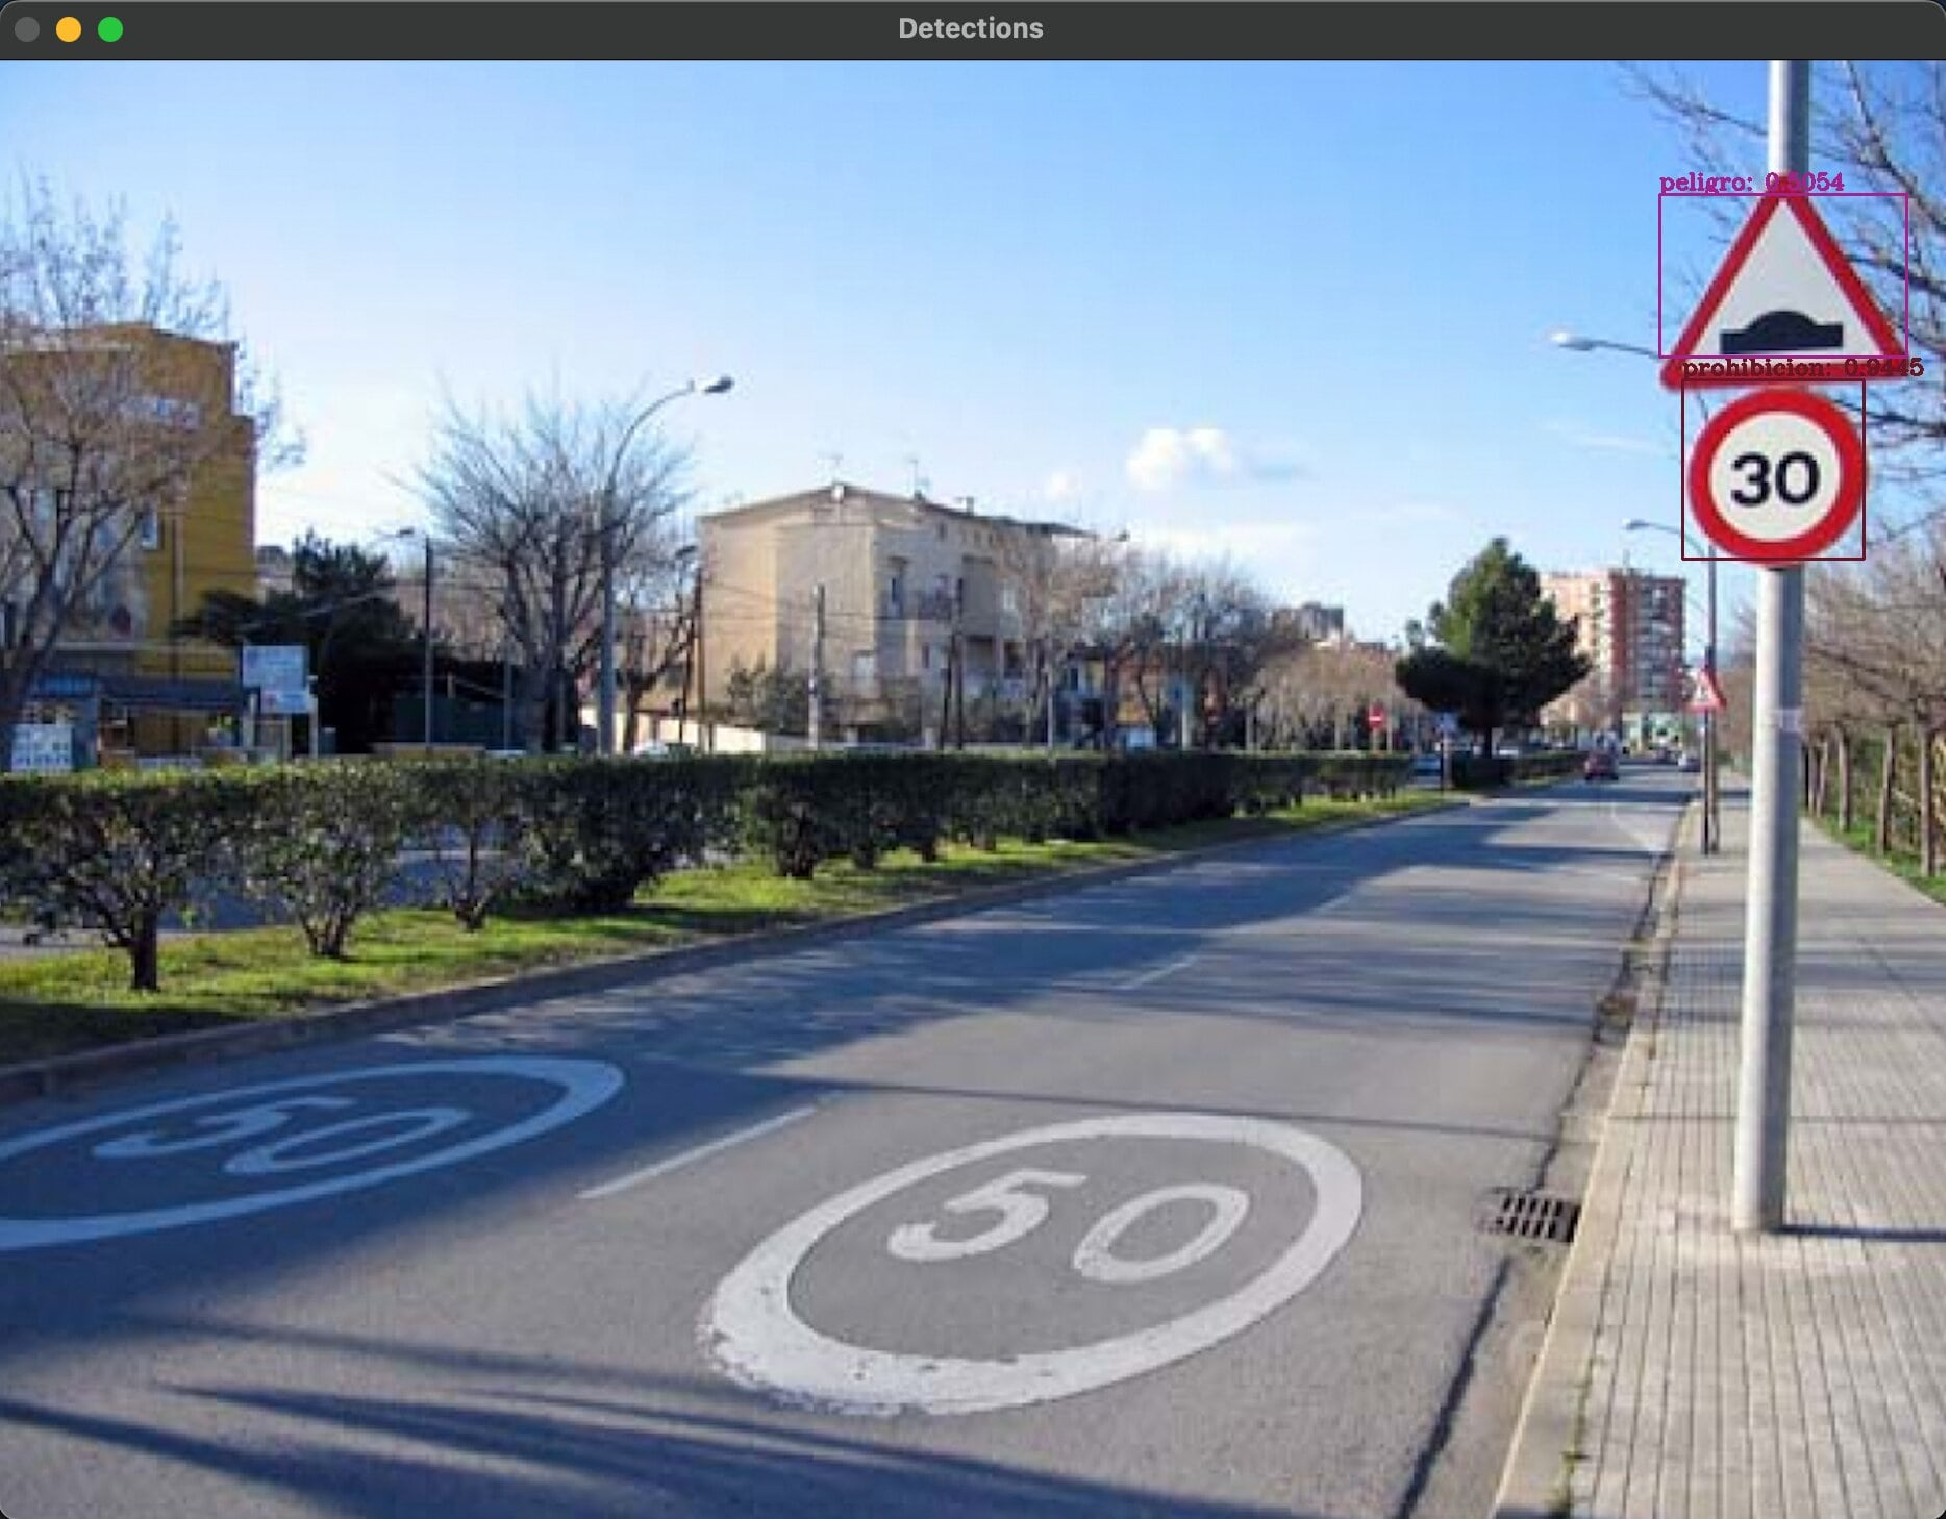
\includegraphics[width=0.6\textwidth]{Imagenes/IA/deteccion3.pdf}
    \caption{Detección de señales reales en vídeo en carretera real}
    \label{deteccion3}
\end{figure}

Finalmente, a través de un popular repositorio de GitHub \url{https://github.com/rafaelpadilla/Object-De\ tection-Metrics.git} dedicado a medir el rendimiento de algoritmos de detección, podremos analizar nuestro sistema de detección de señales. A través de 64 imágenes etiquetadas y procesadas por el algoritmo, podremos medir el rendimiento de la red mediante sus detecciones. En concreto, podremos obtener la curva de Precisión vs Recuperación (Precision vs \textit{Recall}) de nuestro modelo. La precisión es un término que describe la medida verdaderos positivos (TP) en relación con los falsos positivos (FP). Por otro lado, la recuperación se refiere a la proporción de verdaderos positivos (TP) en comparación con la suma de verdaderos positivos y falsos negativos (FN). En resumen, estos conceptos son utilizados para evaluar la efectividad de un modelo de clasificación y se pueden emplear para establecer el límite óptimo del modelo.\\

Para calcular la precisión y la recuperación se hace uso de las siguientes fórmulas:\\
\\
$$\text{precisión} = \frac{\text{TP}}{\text{TP} + \text{FP}}\ \text{recuperación} = \frac{\text{TP}}{\text{TP} + \text{FN}}$$
\\

Podemos contemplar en la figura \ref{rendimiento} que para cada categoría contemplada de señales de tráfico obtenemos una precisión media (AP) diferente. . Establecida una probabilidad mínima de detección de 0,5 y threshold de 0,3, tenemos para la clase obligación se obtiene una precisión del 57,9\%, para peligro un 72,22\%, para prohibición un 84,54\% y para el resto un 62,14\%. Destacar que entre las 64 imágenes que se han analizado, se encontraban tanto imágenes de señales reales, como señales de juguete, esto es clave porque los pesos pre-entrenados no contaban con señales falsas. Por ello, podemos notar que quizás los valores de precisión obtenidos no son suficientemente altos debido a la inclusión de señales que no se asemejan con las de entrenamiento.\\

\begin{figure}[H]
    \centering
 	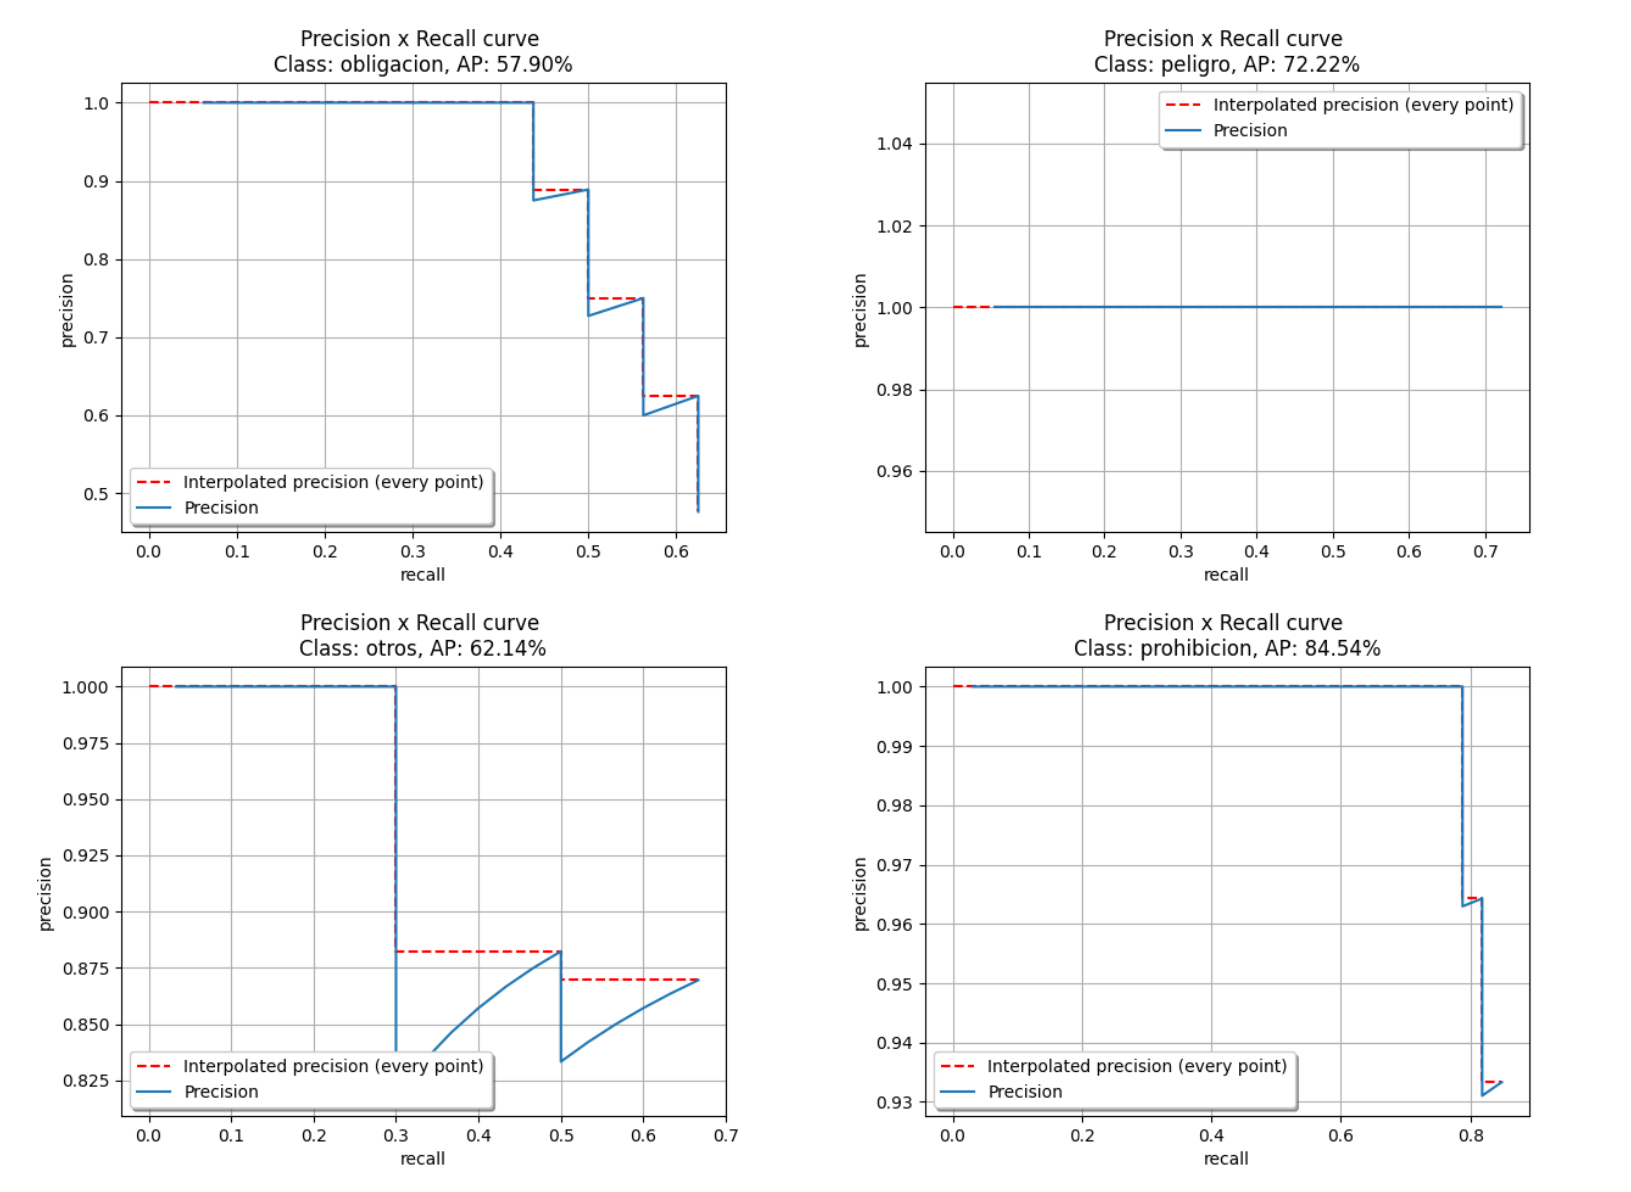
\includegraphics[width=\textwidth]{Imagenes/IA/rendimiento.pdf}
    \caption{Gráficas del rendimiento obtenido}
    \label{rendimiento}
\end{figure}

En primer lugar, en conocimiento de que la mayor precisión la hemos obtenido para la clase prohibición con una probabilidad de casi el 85\%, podemos ver que está cerca de parecerse a la curva ideal. La curva ideal que desearíamos sería una curva que se acerque lo máximo posible a la esquina superior derecha, es decir, alta precisión y alto recall. Asimismo, podemos relacionar la curva ideal con el área bajo la curva de precisión, el valor de precisión media obtenido representa el área bajo dicha curva, por lo que si la curva fuese ideal sería claro que al área sería del 100\%.\\

Podemos concluir entonces que la mejor precisión se ha obtenido en la detección de señales de prohibición. Además, destacar el resultado obtenido para la clase peligro, el cual puede llamar la atención por resultar una línea recta en todo momento. Esto se debe a que para todas las imágenes que se han contemplado para medir el rendimiento, el algoritmo ha sido capaz de detectar todas las señales que se han procesado. Este resultado quizás no sea del todo realista, por lo que se podrían añadir un mayor número de imágenes de cada clase para lograr objetivos más fehacientes con la realidad.\\

Una vez montada la estructura principal del sistema de inteligencia artificial, se procedió a intentar implementar nuevas funcionalidades con el objetivo de mejorar las prestaciones. Se decidió entonces dar un paso más allá en la clasificación de las señales, para intentar detectar de qué tipo de señal concreta se trata.\\

Como ya se ha mencionado, entrenar un algoritmo de IA requiere de una capacidad computacional muy alta. Por ello, una forma sencilla de implementar cierta inteligencia que sea capaz de detectar las señales tras procesarlas mediante YOLO, sería la incorporación de una red CNN.\\

Una CNN o Convolutional Neural Network (Red Neuronal Convolucional) es un tipo de arquitectura de red neuronal especialmente diseñada para procesar datos, como imágenes o audio. Ésta destaca por su rendimiento en visión artificial gracias a su capacidad para capturar características locales y patrones espaciales en imágenes, es decir, detección y clasificación de objetos.\\

La consecución de ambas tecnologías, tal y como se ejemplifica en la figura \ref{esquema}, nos permite ciertas ventajas en la consecución de ambas tecnologías:\\

\begin{itemize}
\item 1.	Eficiencia: YOLO destaca por su eficiencia en la detección de objetos, por lo que hacer una detección inicial nos permitirá identificar rápidamente las ubicaciones aproximadas de las señales de tráfico.
\item 2.	Localización precisa: Una vez que YOLO detecta las señales de tráfico, la ubicación de la señal se utiliza para extraer una región más pequeña, que es enviada a las CNN correspondientes para una clasificación más precisa. Al hacer esto, te aseguras de que solo se envíen las regiones relevantes a las CNN, en lugar de toda la imagen, lo que ayuda a mejorar la eficiencia y precisión del proceso de clasificación.
\item 3.	Especialización: Al entrenar las CNN separadas para cada categoría específica de señales de tráfico, logramos una especialización en la clasificación. Como cada CNN se entrena con imágenes específicas, permite una mayor capacidad para aprender características distintivas y patrones asociados a cada tipo de señal.
\end{itemize}

\begin{figure}[H]
    \centering
 	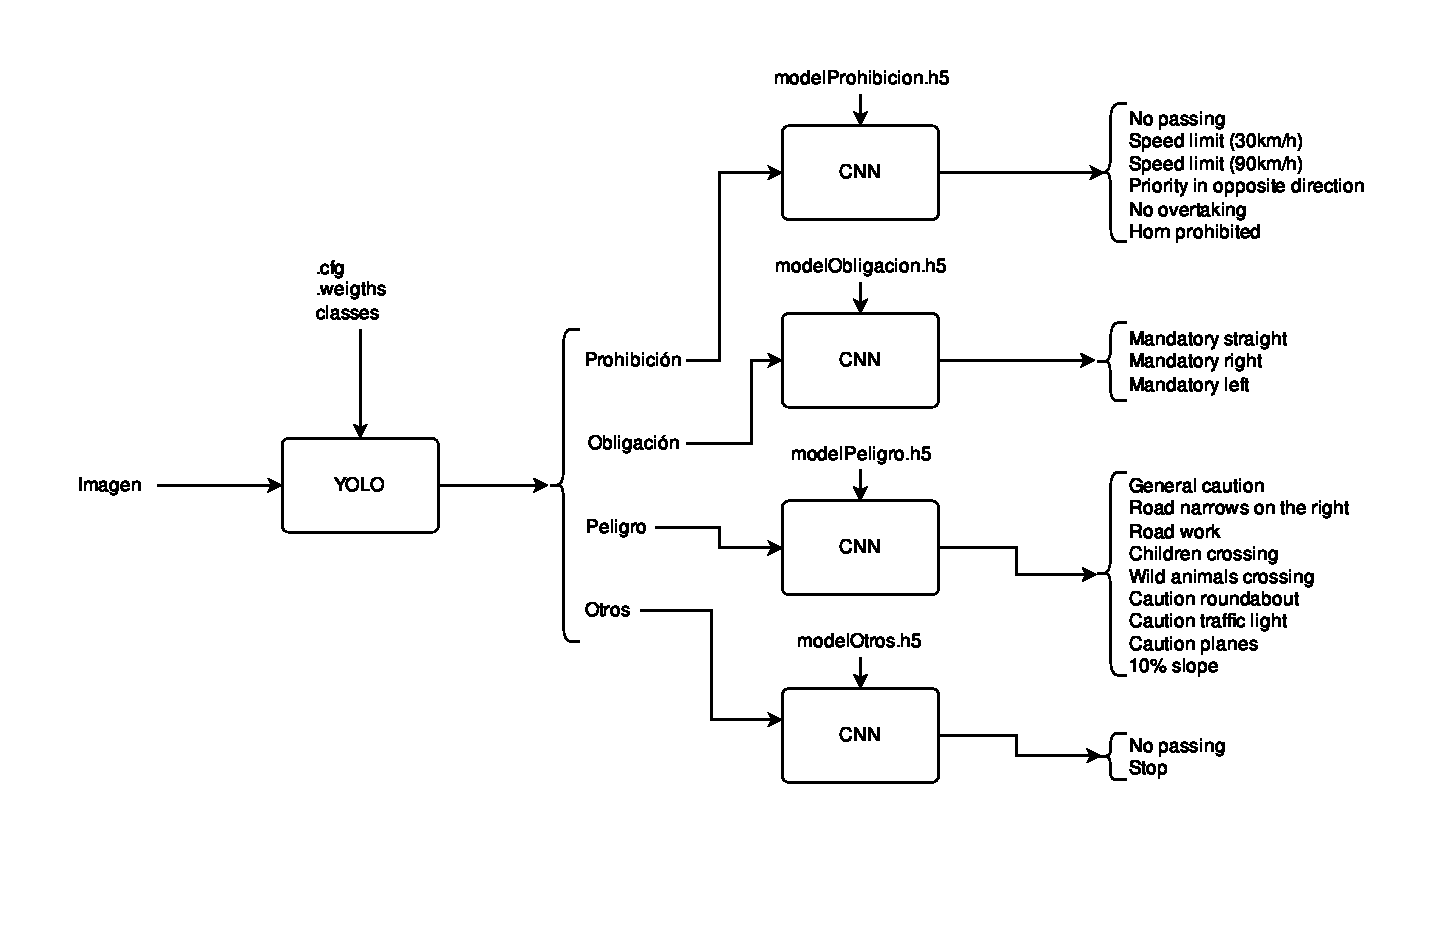
\includegraphics[width=\textwidth]{Imagenes/IA/EsquemaIA.pdf}
    \caption{Ventajas de las diferentes tecnologías}
    \label{esquema}
\end{figure}

El modelo CNN definido consta de varias capas. La estructura de capas que contiene el modelo son las siguientes:\\

\begin{itemize}
\item 1.	Capa de convolución 2D con 16 filtros y tamaño de kernel 3x3, con función de activación ReLU.
\item 2.	Capa de convolución 2D con 32 filtros y tamaño de kernel 3x3, con función de activación ReLU.
\item 3.	Capa de MaxPooling 2D con tamaño de pool 2x2.
\item 4.	Capa de normalización por lotes (Batch Normalization).
\item 5.	Capa de convolución 2D con 64 filtros y tamaño de kernel 3x3, con función de activación ReLU.
\item 6.	Capa de convolución 2D con 128 filtros y tamaño de kernel 3x3, con función de activación ReLU.
\item 7.	Capa de MaxPooling 2D con tamaño de pool 2x2.
\item 8.	Capa de normalización por lotes (Batch Normalization).
\item 9.	Capa de aplanamiento (Flatten).
\item 10.Capa densa (fully connected) con 512 neuronas y función de activación ReLU.
\item 11.Capa de normalización por lotes (Batch Normalization).
\item 12.Capa de Dropout con una tasa de dropout de 0.5.
\item 13.Capa densa (fully connected) con 2 neuronas y función de activación softmax.
\end{itemize}


En total, las CNNs están formadas 13 capas, incluyendo las capas de convolución, capas de pooling, capas de normalización por lotes, capas densas y capas de dropout. Cada una de estas capas realiza las siguientes funciones:\\

\begin{itemize}
\item 1.	Capa de convolución 2D: Realiza la convolución de la imagen de entrada con un conjunto de filtros para extraer características importantes de la imagen. Utiliza una función de activación ReLU para introducir no linealidad en la red.
\item 2.	Capa de convolución 2D: Similar a la capa anterior, realiza otra convolución con un conjunto de filtros diferentes para extraer más características de la imagen. También utiliza la función de activación ReLU.
\item 3.	Capa de MaxPooling 2D: Reduce la dimensión espacial de la salida de las capas anteriores mediante la reducción de la resolución espacial. Ayuda a disminuir la cantidad de parámetros y a aprender características más generales.
\item 4.	Capa de normalización por lotes (Batch Normalization): Normaliza los valores de activación de la capa anterior para acelerar el entrenamiento y mejorar la estabilidad de la red.
\item 5.	Capa de convolución 2D: Realiza otra convolución con más filtros para extraer características más complejas de la imagen.
\item 6.	Capa de convolución 2D: Realiza otra convolución con aún más filtros para capturar características más específicas de la imagen.
\item 7.	Capa de MaxPooling 2D: Reduce la dimensión espacial de la salida de las capas anteriores.
\item 8.	Capa de normalización por lotes (Batch Normalization): Normaliza los valores de activación de la capa anterior.
\item 9.	Capa de aplanamiento (Flatten): Transforma la salida de la capa anterior en un vector unidimensional, preparándola para la entrada a las capas densas.
\item 10.Capa densa (fully connected): Capa de neuronas completamente conectadas donde cada neurona está conectada a todas las neuronas de la capa anterior. Utiliza la función de activación ReLU.
\item 11.Capa de normalización por lotes (Batch Normalization): Normaliza los valores de activación de la capa anterior.
\item 12.Capa de Dropout: Apaga aleatoriamente un porcentaje de las neuronas durante el entrenamiento para evitar el sobreajuste y mejorar la generalización del modelo.
\item 13.Capa densa (fully connected): Capa final de clasificación con 2 neuronas y función de activación softmax. Produce las probabilidades de pertenencia a cada una de las subclases.
\end{itemize}


Fruto del entrenamiento hemos obtenido las matrices de confusión de cada CNN, en una matriz de confusión las filas representan las clases reales y las columnas representan las clases predichas por el modelo, donde cada celda de la matriz muestra la cantidad de ejemplos que pertenecen a una clase específica. La estructura general de este tipo de matrices es la siguiente \ref{genconf} \cite{cm}\\

\begin{figure}[H]
    \centering
 	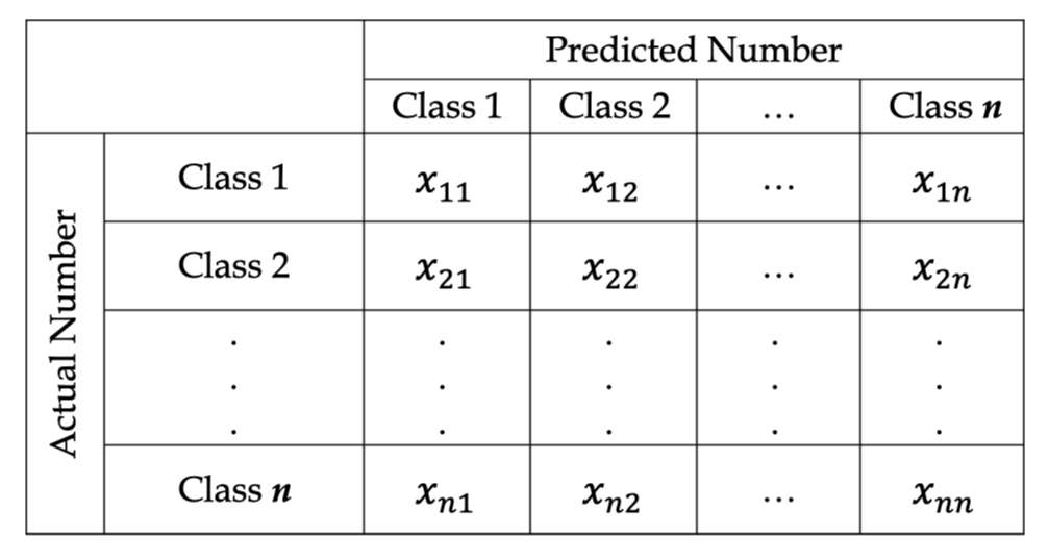
\includegraphics[width=\textwidth]{Imagenes/IA/general_confusion.pdf}
    \caption{Estructura general de las matrices de confusión}
    \label{genconf}
\end{figure}

Donde el número total de falsos negativos (TFN), falsos positivos (TFP), verdaderos negativos (TTN) y verdaderos positivos son respectivamente (TTP) \ref{forconf}.\\

\begin{figure}[H]
    \centering
 	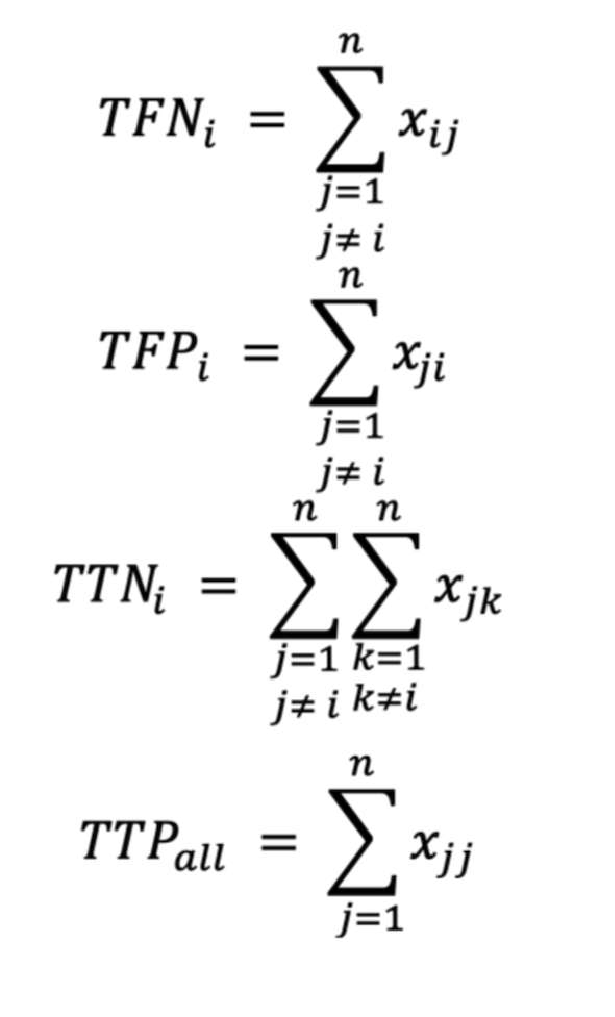
\includegraphics[width=0.2\textwidth]{Imagenes/IA/formulas_confusion.pdf}
    \caption{Fórmulas de cálculo}
    \label{forconf}
\end{figure}

La categoría peligro se divide en 9 subclases: General caution, Road narrows on the right, Road work, Children crossing, Wild animals crossing, Caution roundabout, Caution traffic light, Caution planes y 10\% slope. En su matriz de confusión, encontrada en la figura \ref{pelconf}, detectamos que no se ha producido ninguna detección falsa y que el número de verdaderos positivos es elevado, es decir, el modelo entrenado para las clases de peligro está teniendo un rendimiento muy bueno en términos de clasificación.\\

\begin{figure}[H]
    \centering
 	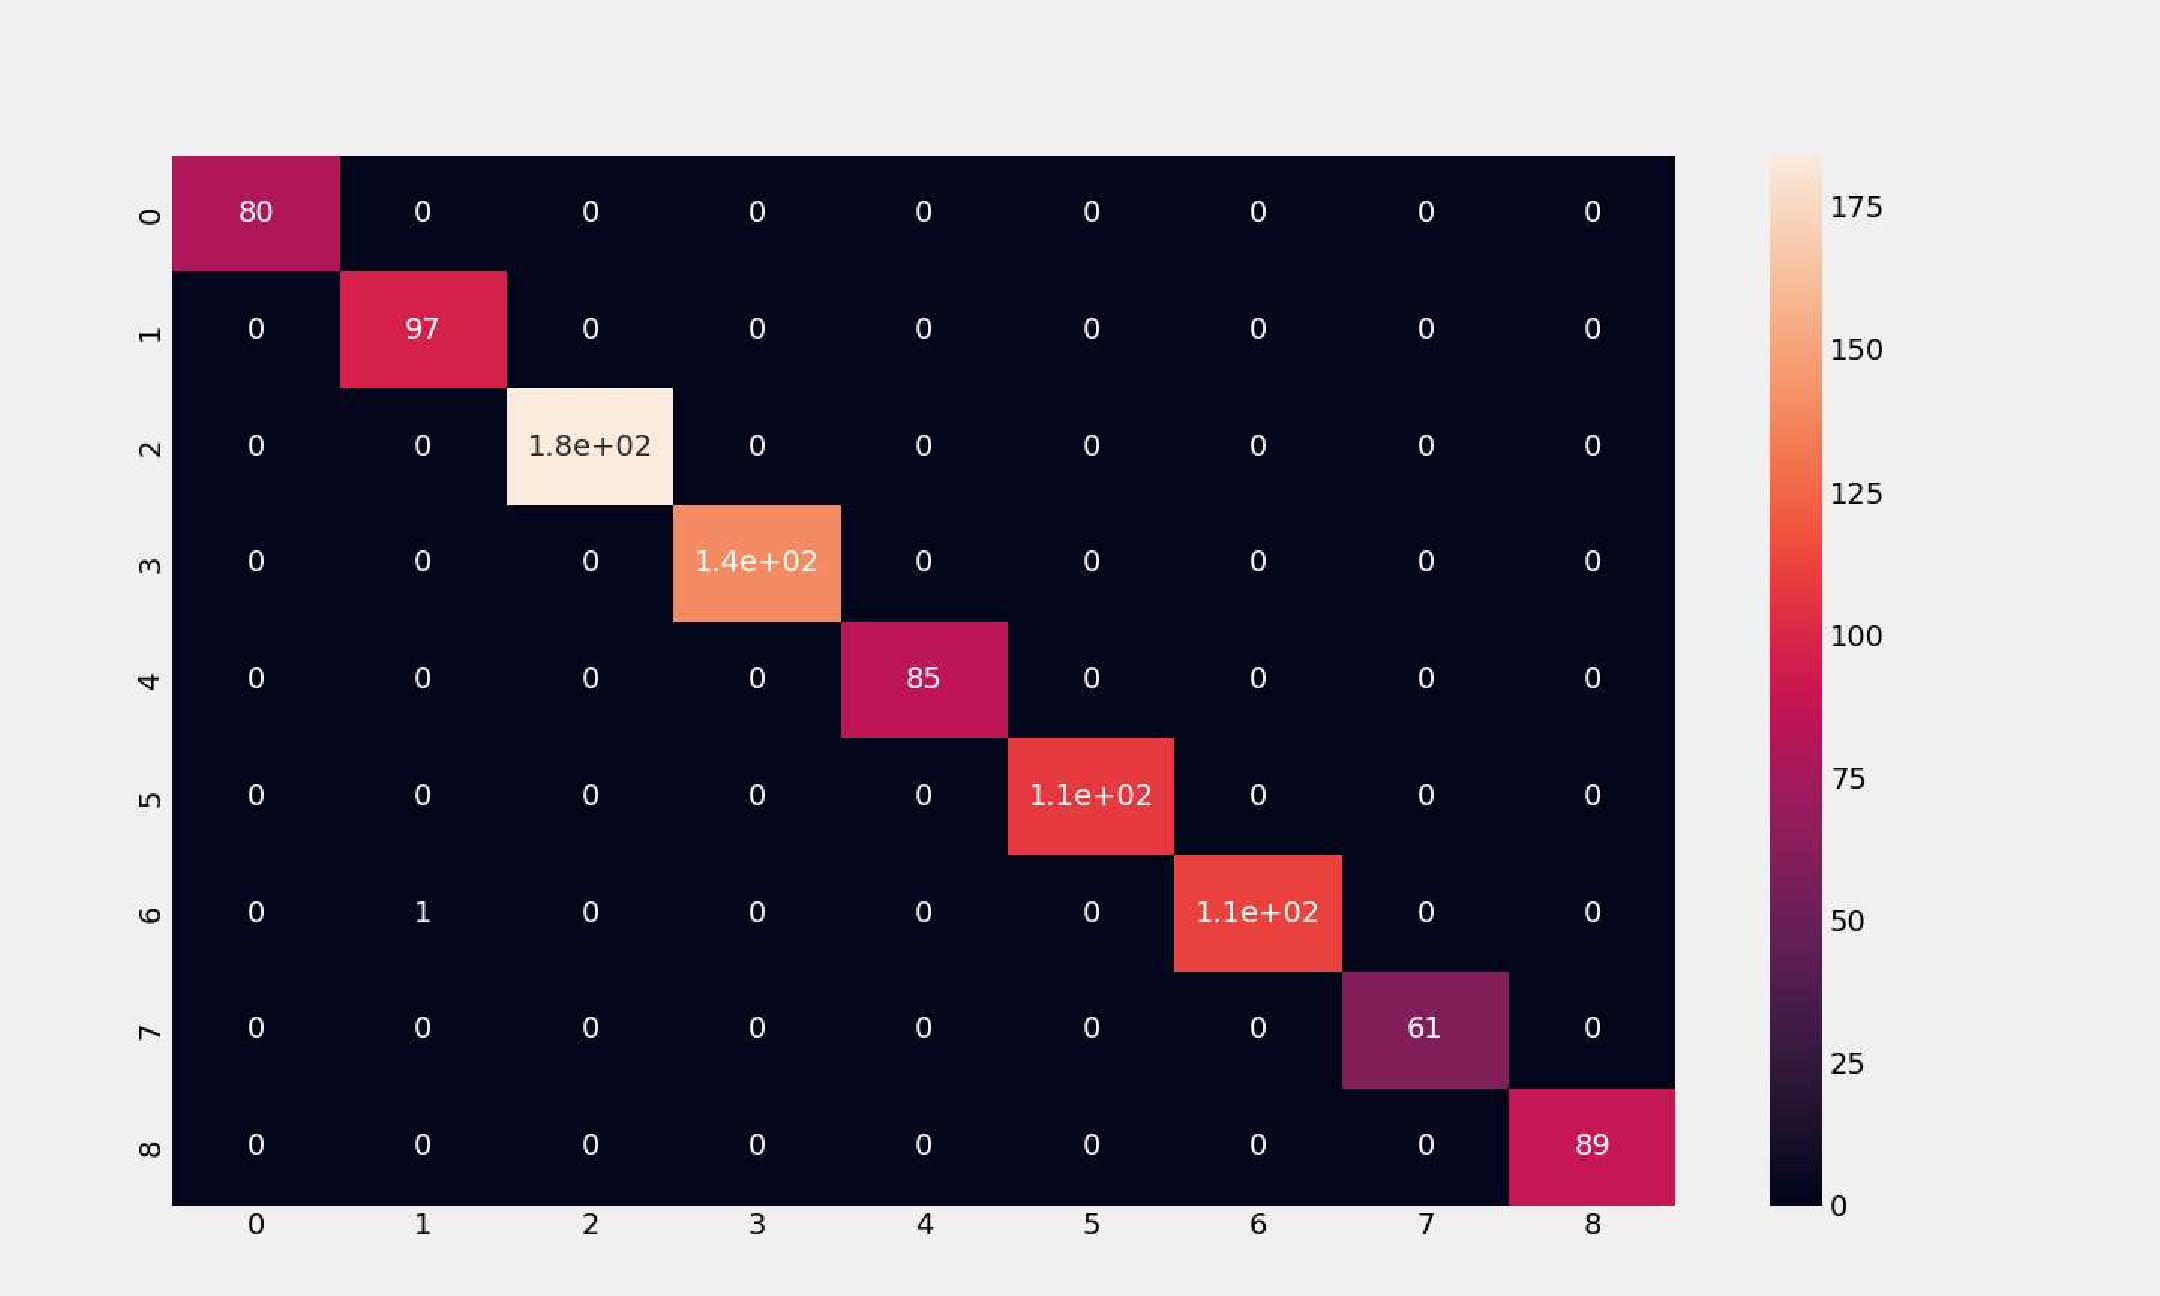
\includegraphics[width=\textwidth]{Imagenes/IA/peligro_confusion.pdf}
    \caption{Matriz de confusión para la categoría peligro}
    \label{pelconf}
\end{figure}

La categoría obligación se divide en 3 subclases: Mandatory straight, Mandatory right y Mandatory left. En la figura \ref{obconf} podemos ver su matriz de confusión, los resultados son análogos a los observados en las clases comentadas para la categoría peligro.\\

\begin{figure}[H]
    \centering
 	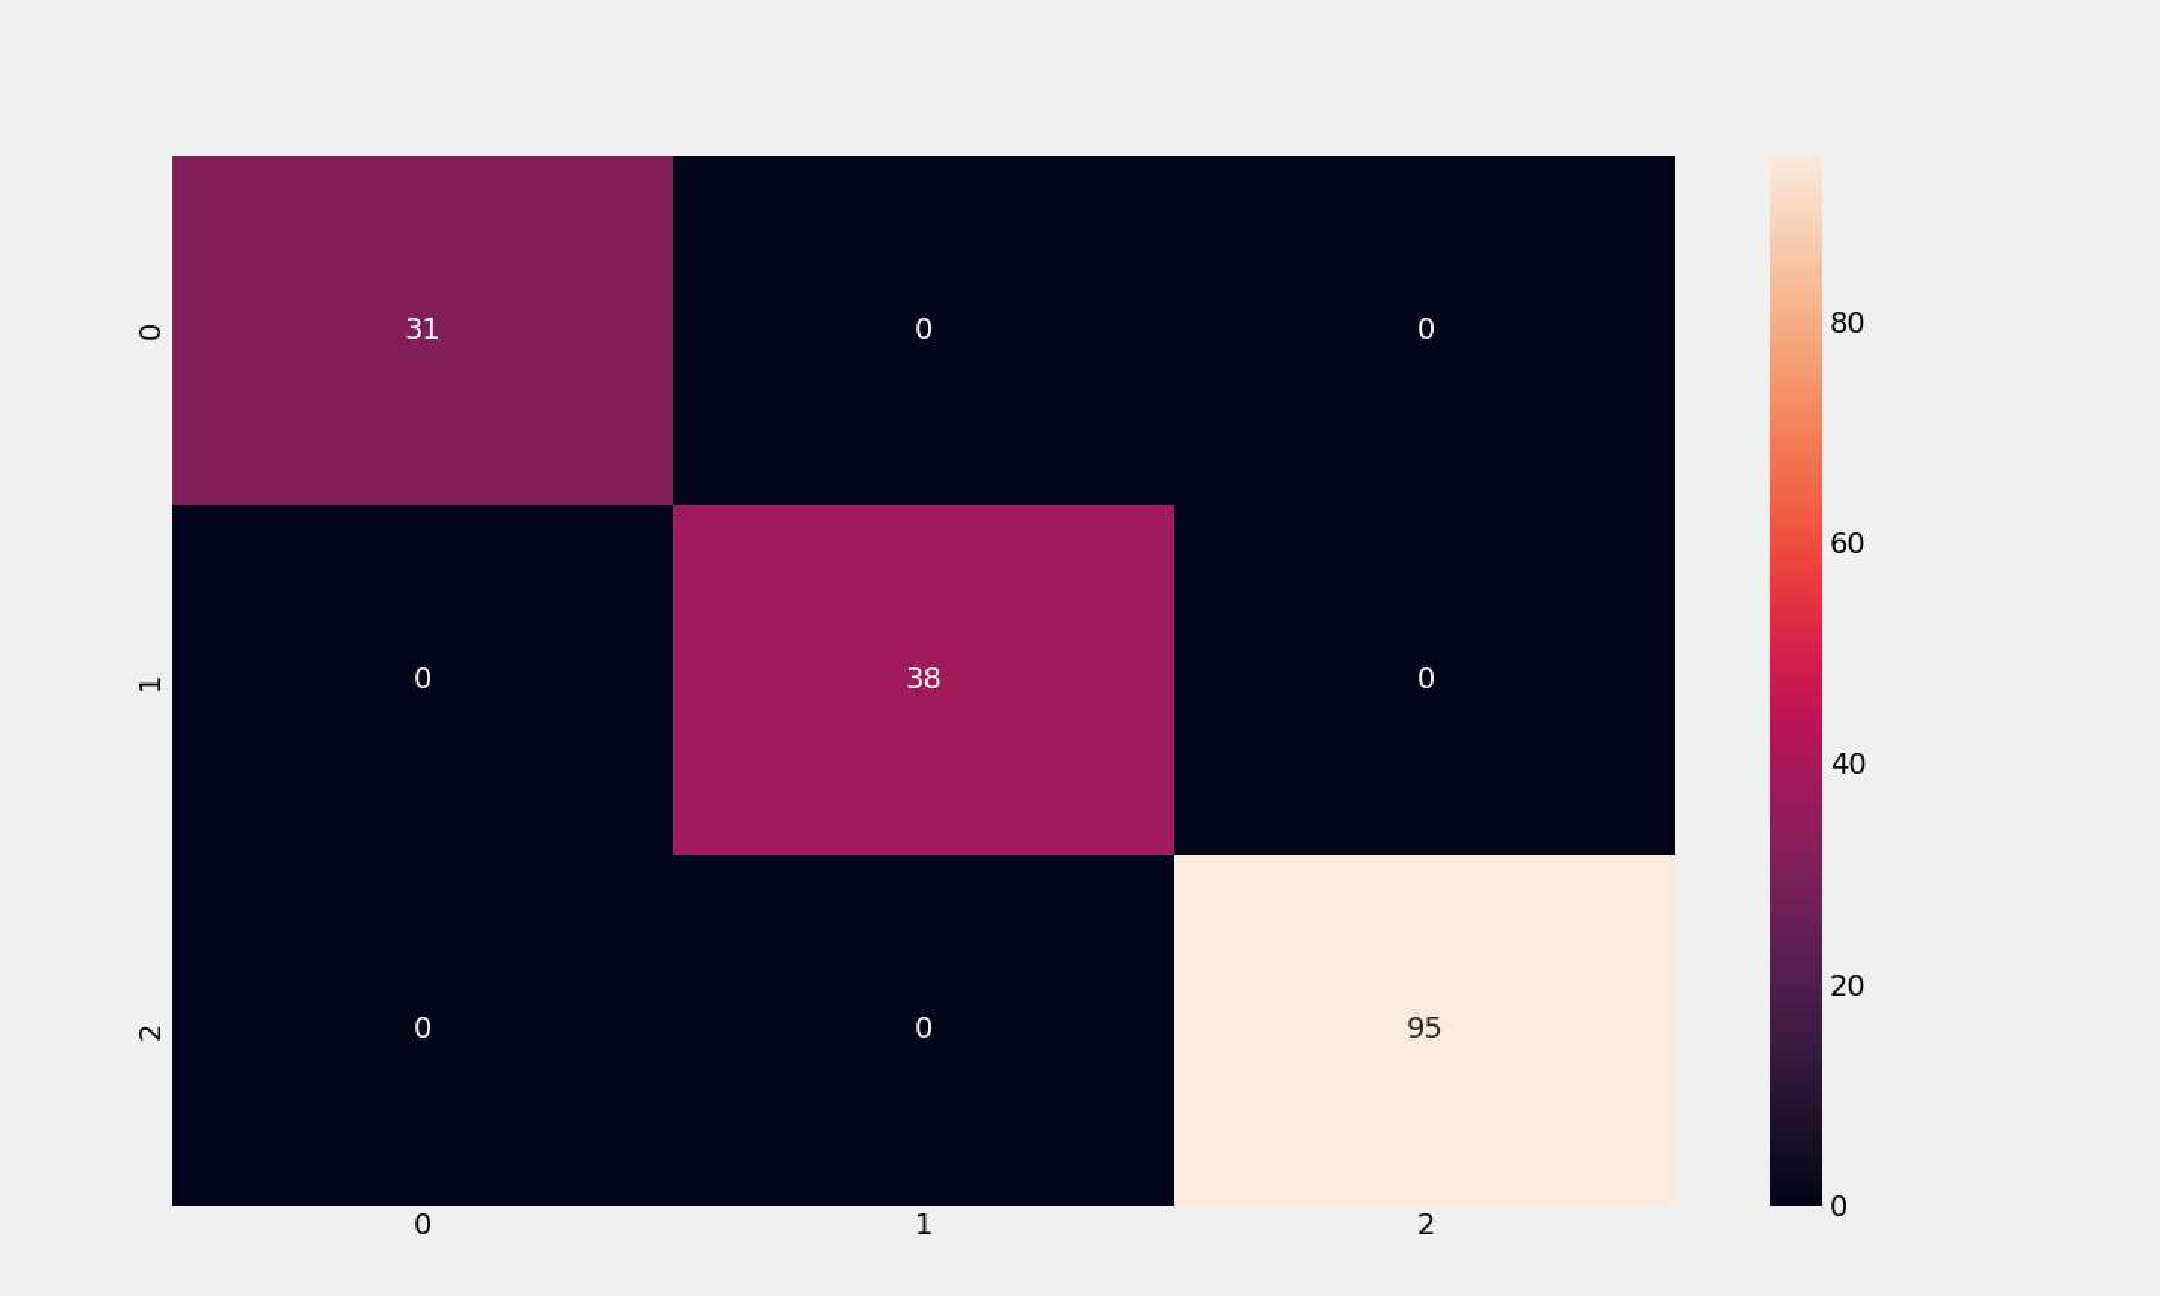
\includegraphics[width=\textwidth]{Imagenes/IA/obligacion_confusion.pdf}
    \caption{Matriz de confusión para la categoría obligación}
    \label{obconf}
\end{figure}

La tercera de las clases que tenemos tras la detección en YOLO es prohibición, que se divide en 6 subclases: No passing, Speed limit (30km/h), Speed limit (90km/h), Priority in opposite direction, No overtaking, Horn prohibited. Analizando los resultados de la figura \ref{probconf} nos damos cuenta de que por primera vez nos encontramos detecciones falsas, sin embargo, la cifra es anecdótica comparada con las detecciones verdaderas.\\

\begin{figure}[H]
    \centering
 	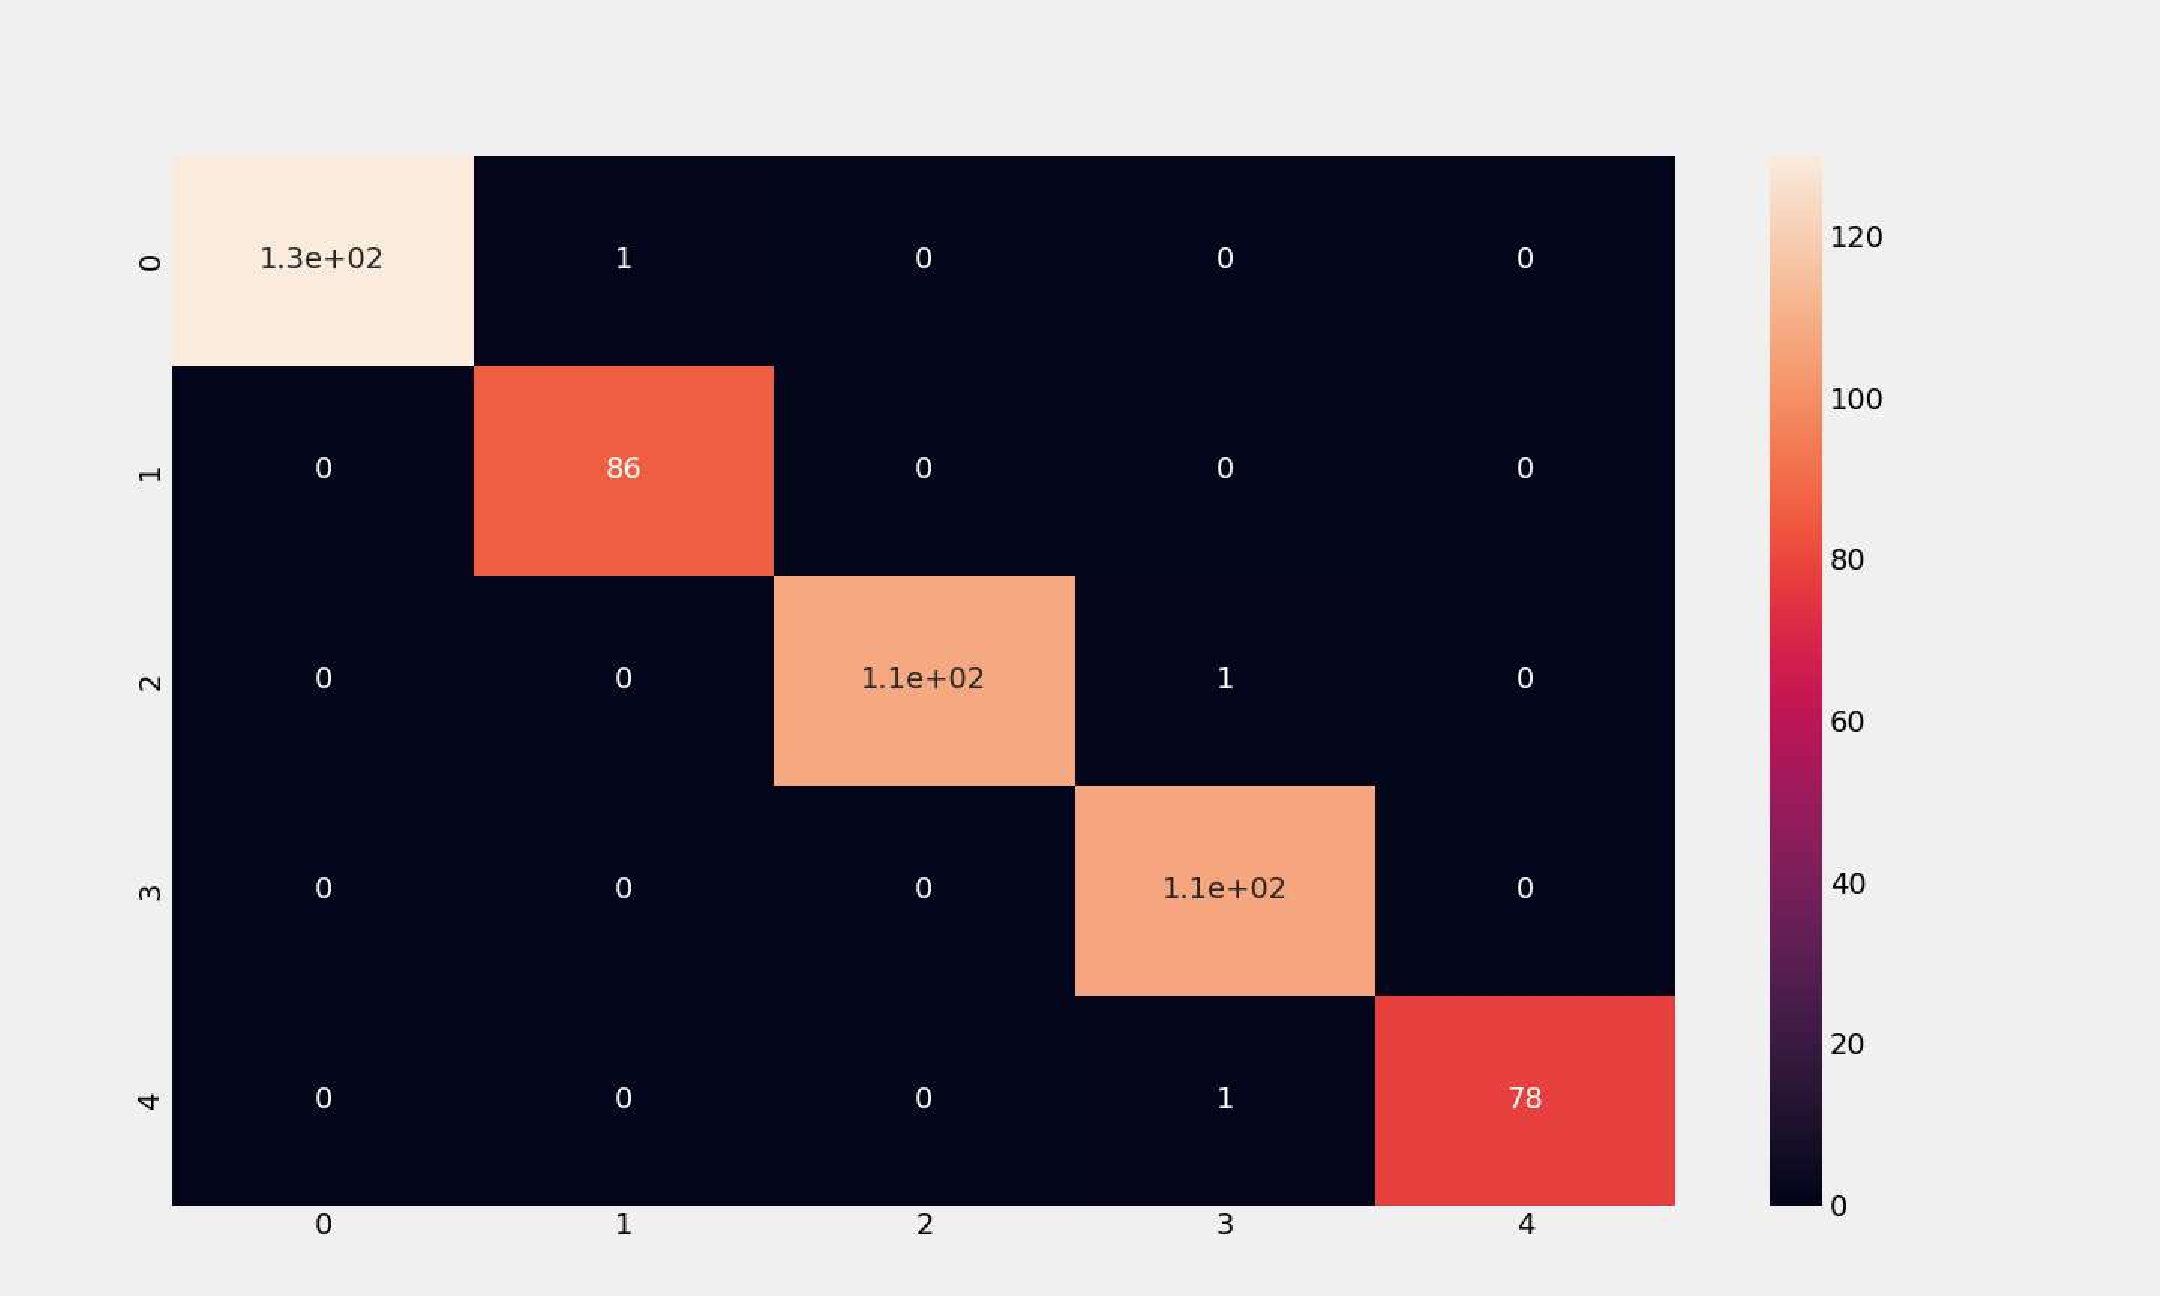
\includegraphics[width=\textwidth]{Imagenes/IA/prohibicion_confusion.pdf}
    \caption{Matriz de confusión para la categoría prohibición.}
    \label{probconf}
\end{figure}

Finalmente, la última clase otros se divide en 2 subclases: No passing y Stop y los resultados son equivalentes a los tres anteriores \ref{otrosconf}.\\

\begin{figure}[H]
    \centering
 	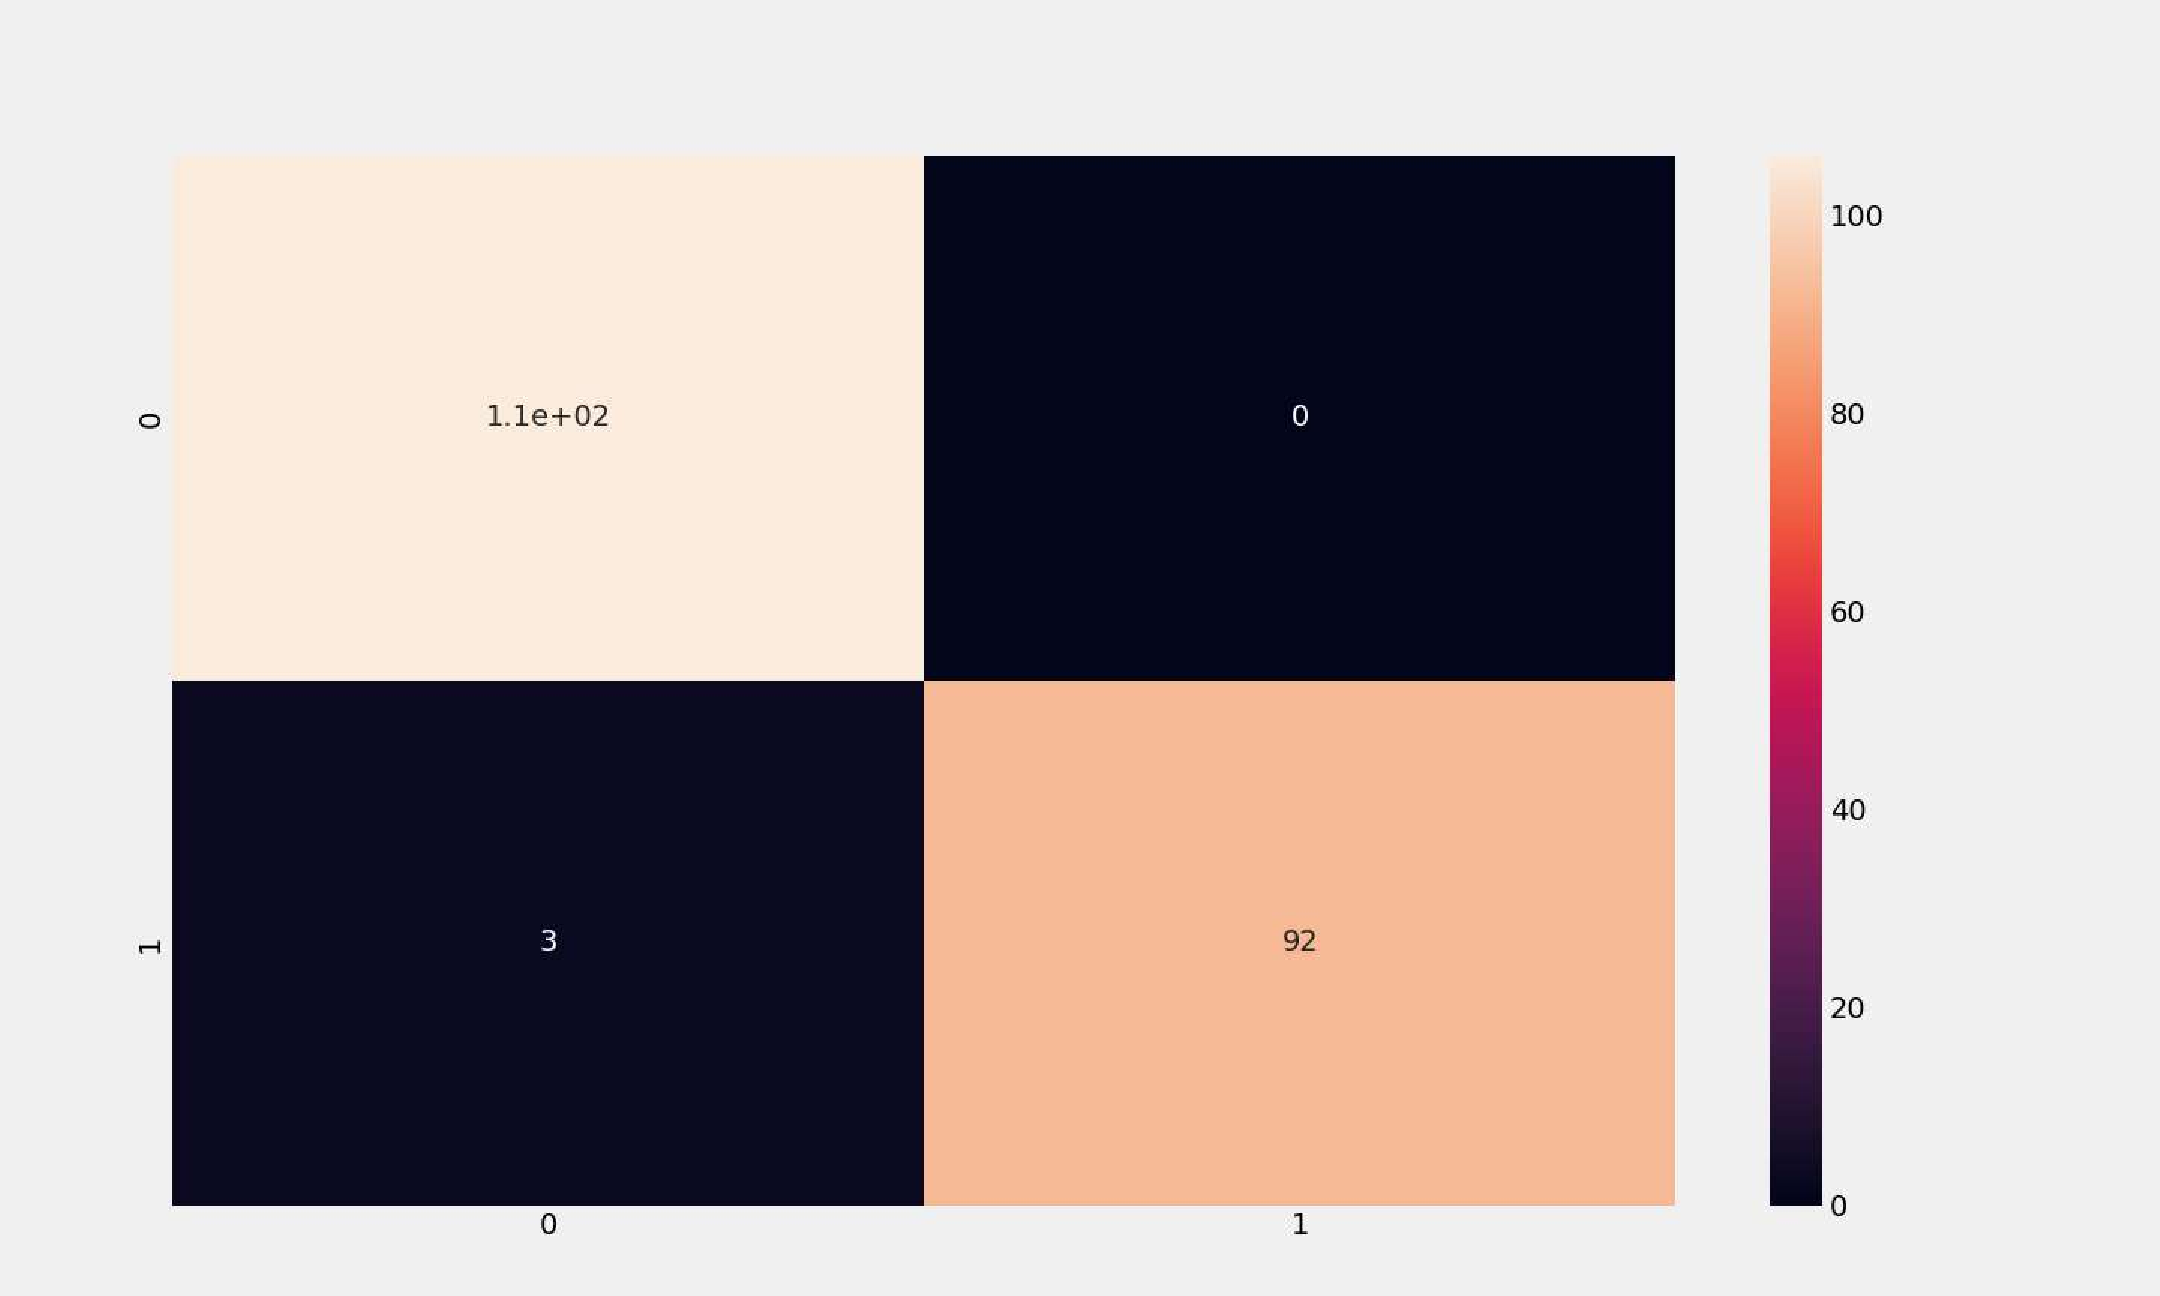
\includegraphics[width=\textwidth]{Imagenes/IA/otros_confusion.pdf}
    \caption{Matriz de confusión para la útltima categoría.}
    \label{otrosconf}
\end{figure}


Llevando a la práctica la incorporación de las redes CNN veremos realmente si son fiables, por ello, procederemos a ver cómo se desenvuelve en el propio vehículo de Amazon. Montando una prueba con el coche y varías señales nos encontramos con los siguientes resultados \ref{c1}, \ref{c2}, \ref{c3}, \ref{c4}.\\

\begin{figure}[H]
    \centering
 	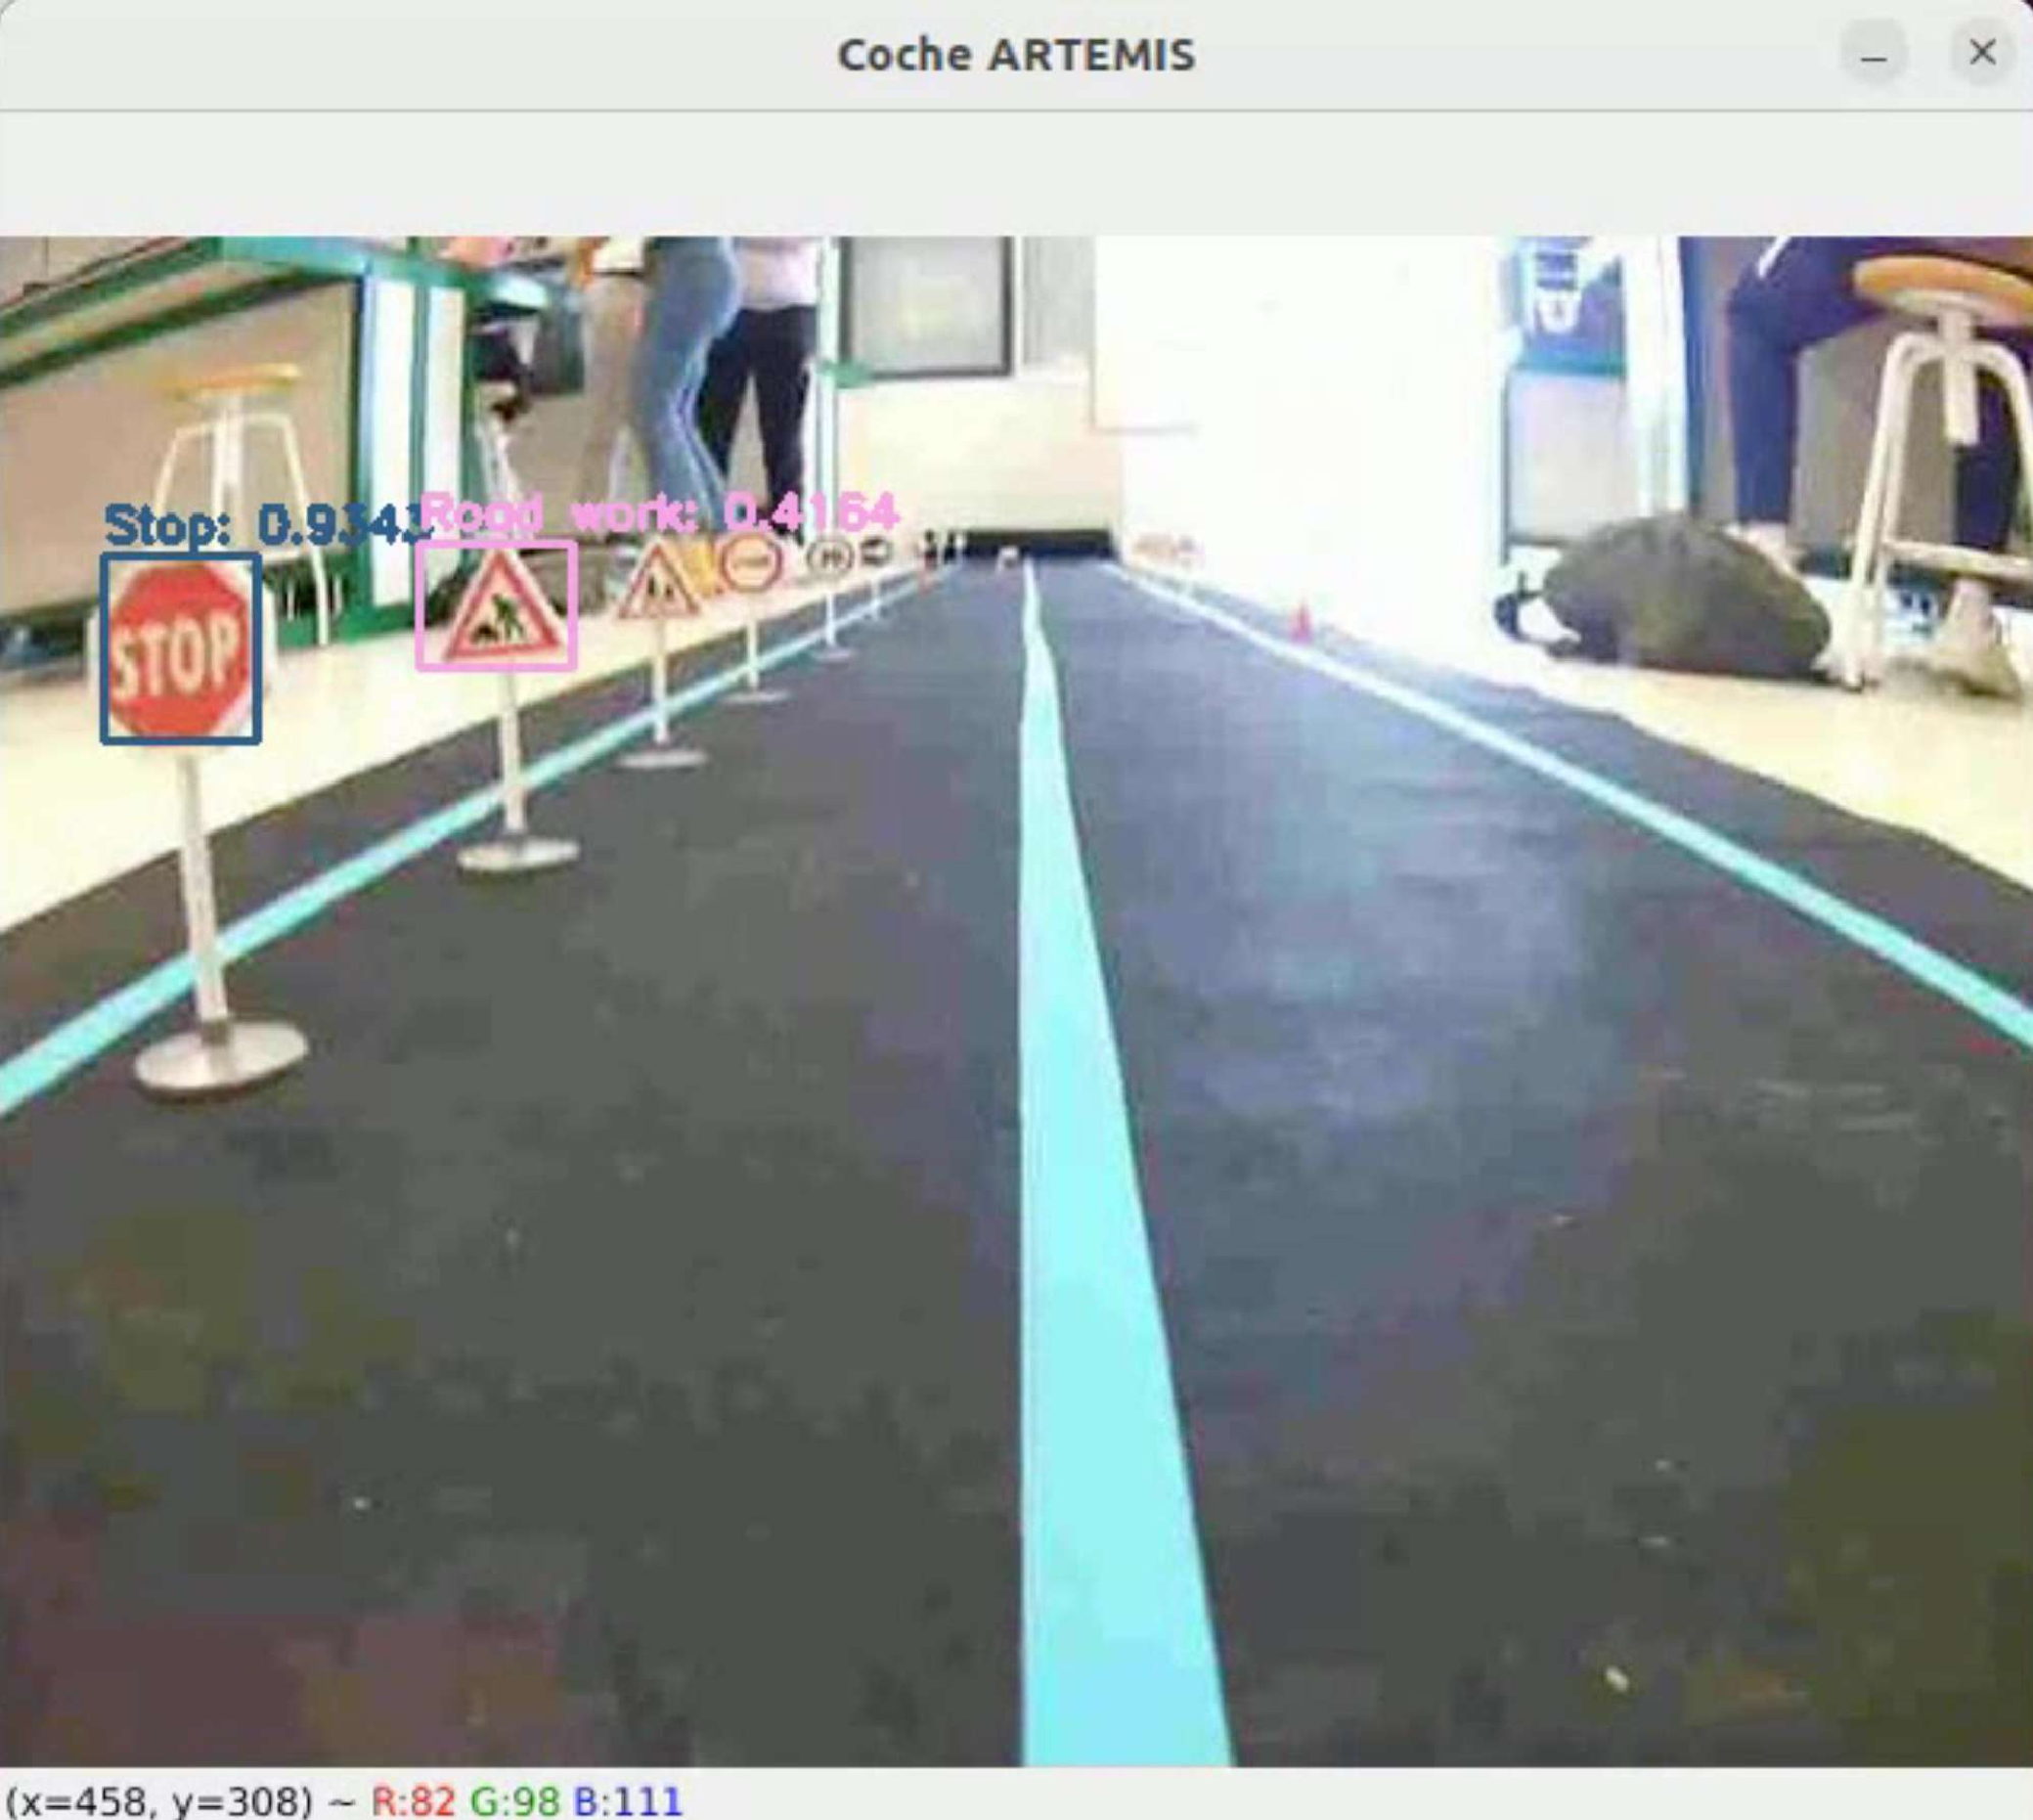
\includegraphics[width=\textwidth]{Imagenes/IA/YoloCNN_coche.pdf}
    \caption{Resultados de la prueba (1).}
    \label{c1}
\end{figure}


\begin{figure}[H]
    \centering
 	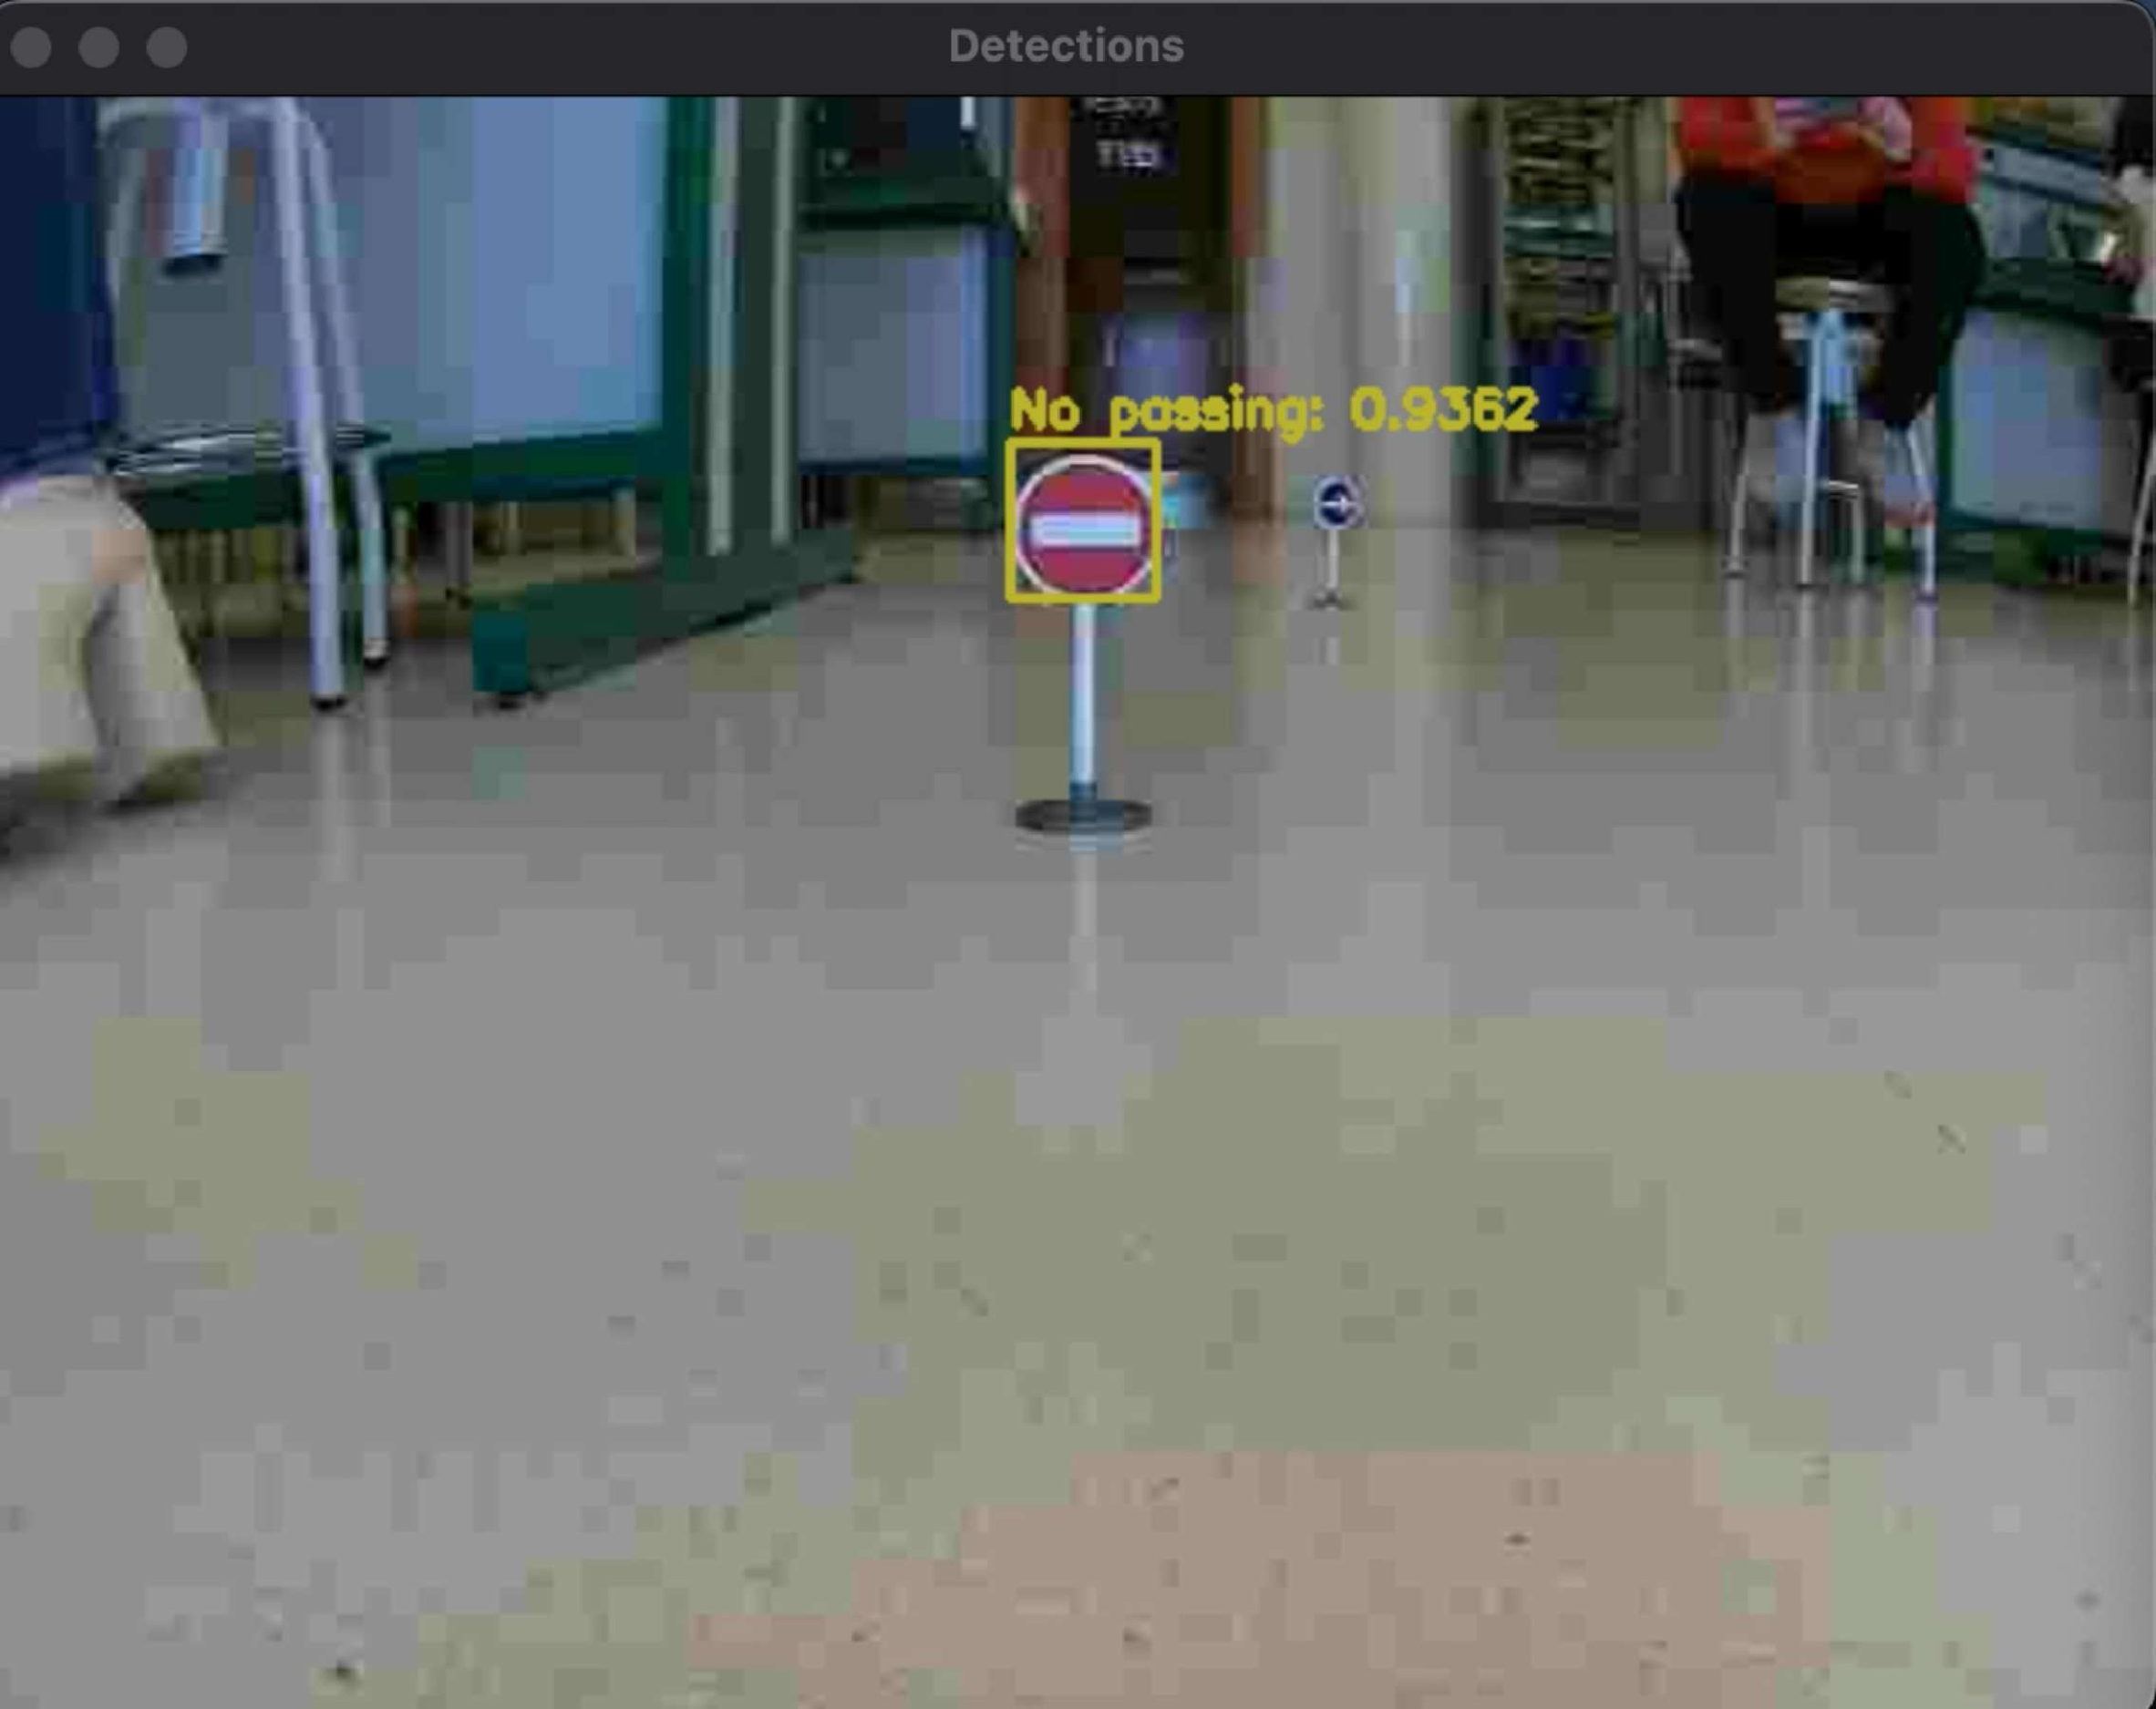
\includegraphics[width=\textwidth]{Imagenes/IA/YoloCNN_coche2.pdf}
    \caption{Resultados de la prueba (2).}
    \label{c2}
\end{figure}

\begin{figure}[H]
    \centering
 	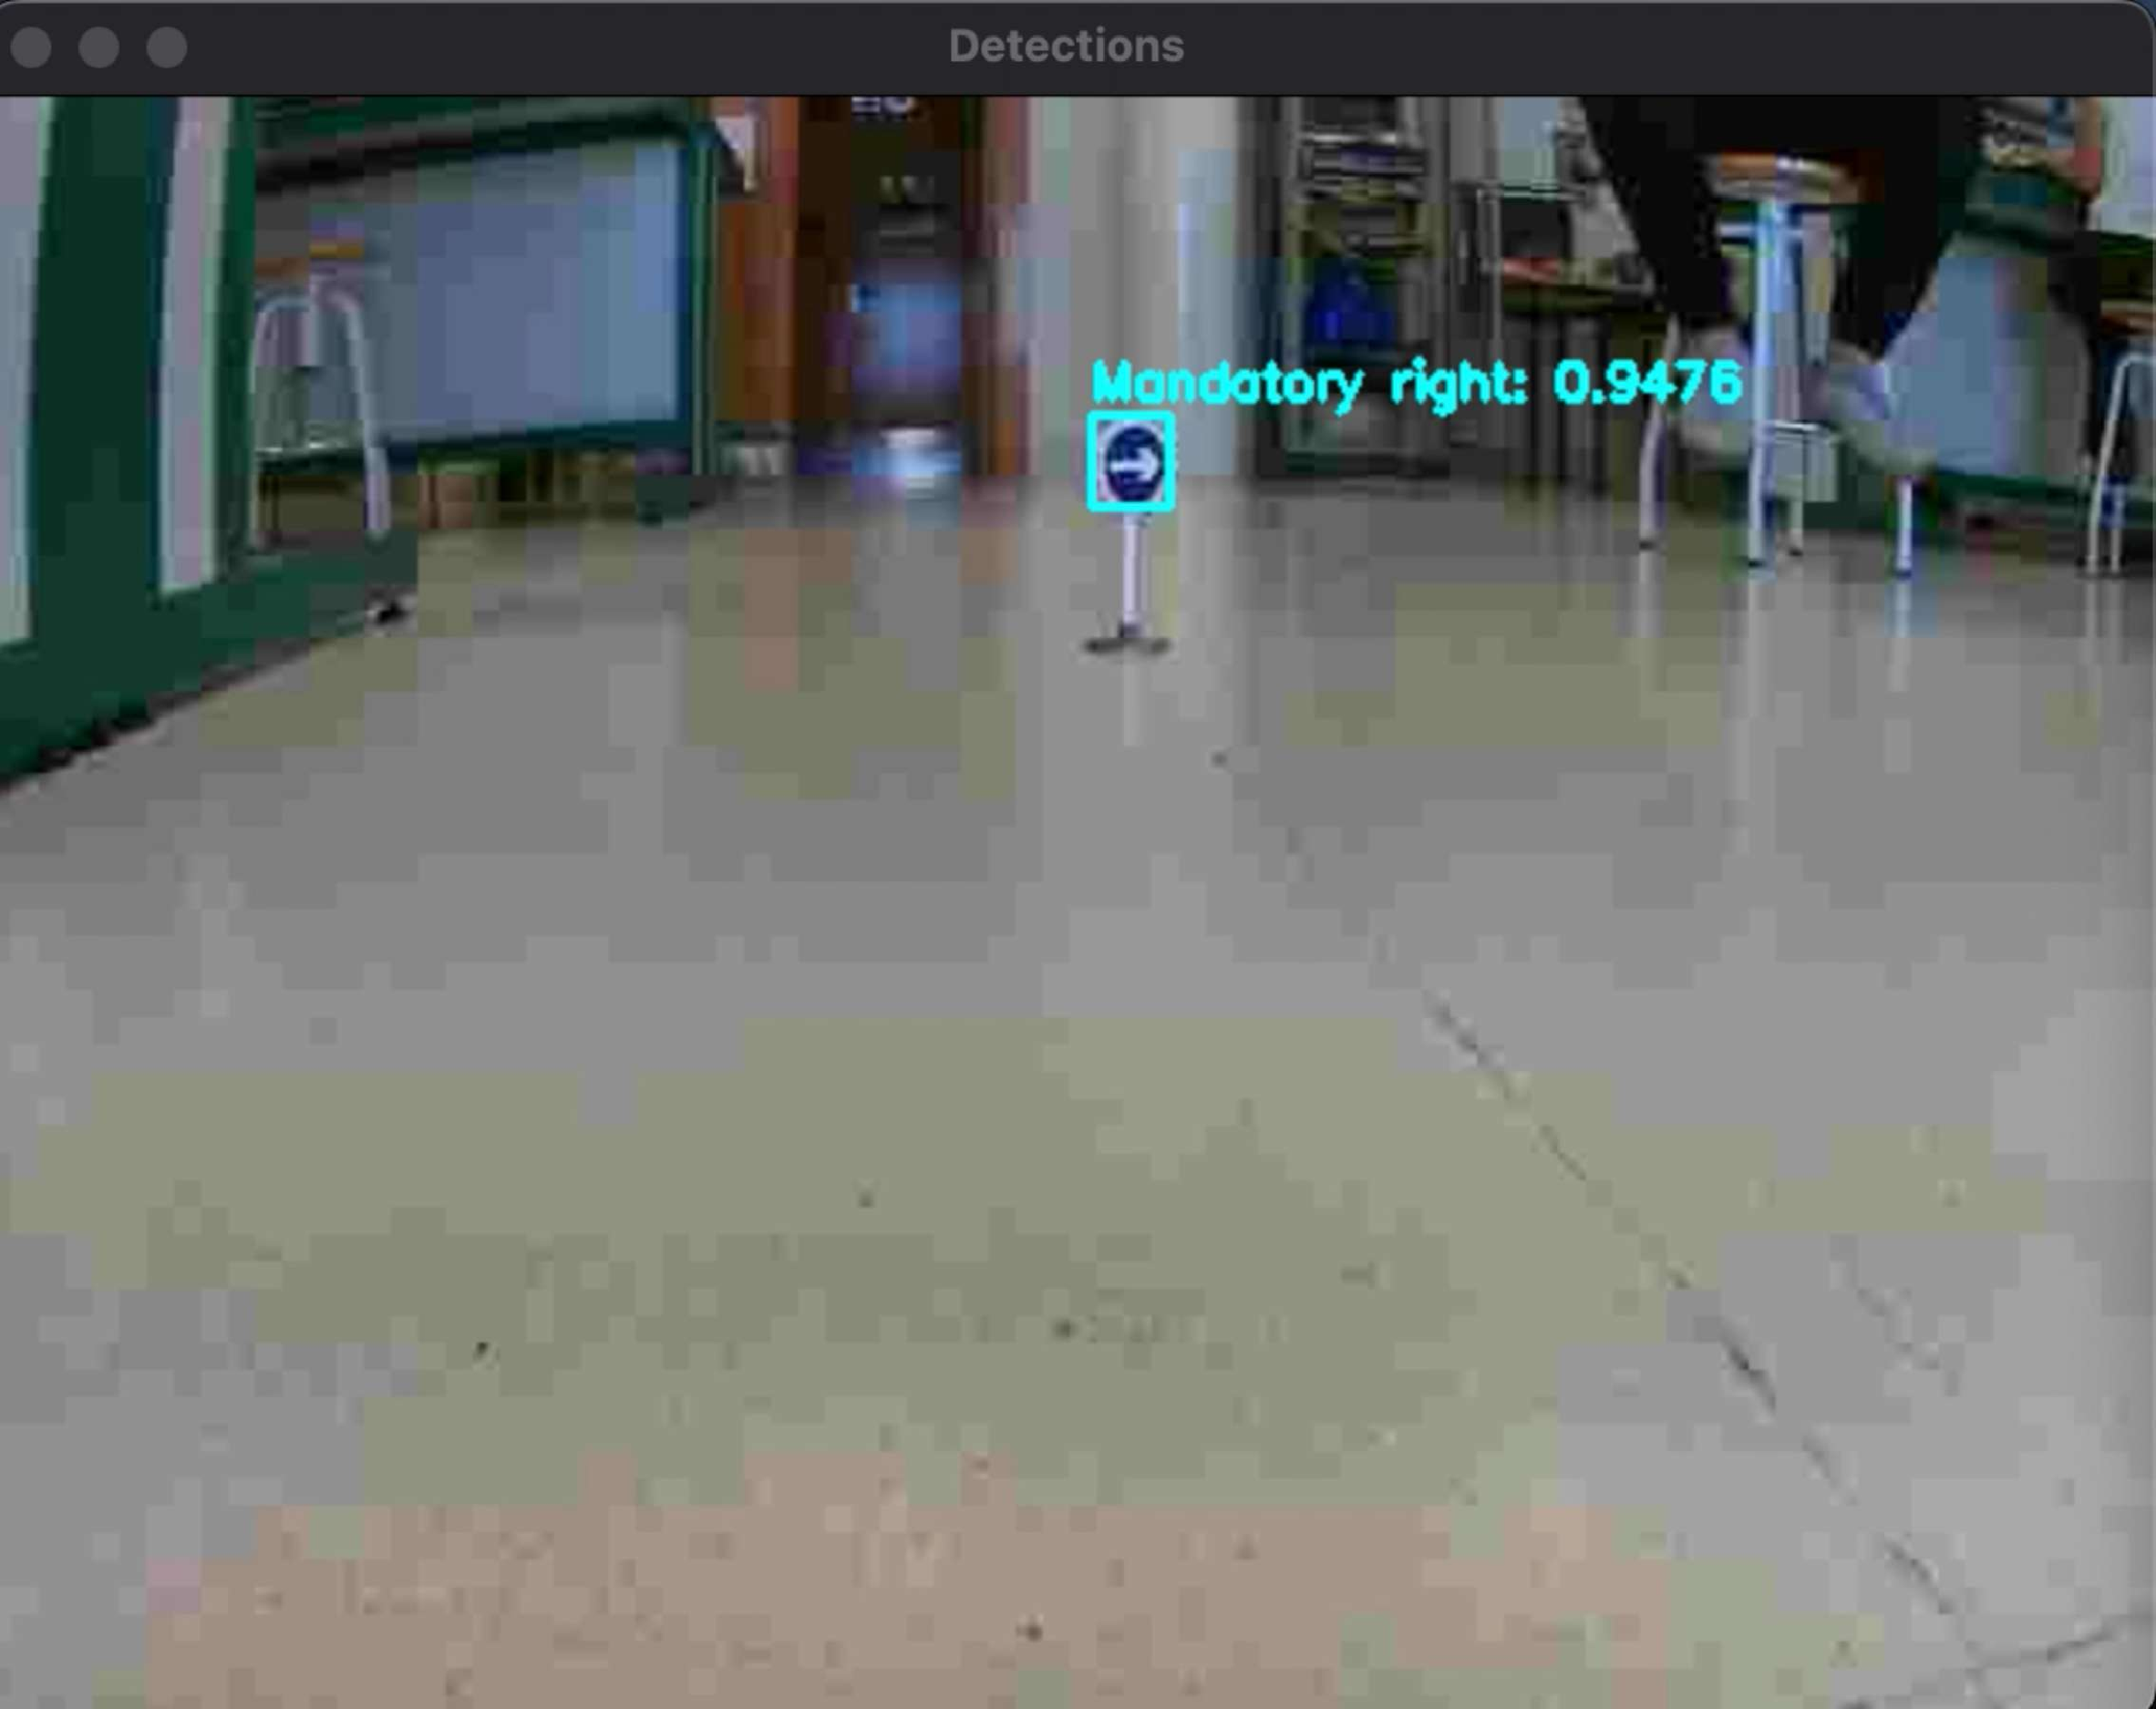
\includegraphics[width=\textwidth]{Imagenes/IA/YoloCNN_coche3.pdf}
    \caption{Resultados de la prueba (3).}
    \label{c3}
\end{figure}

\begin{figure}[H]
    \centering
 	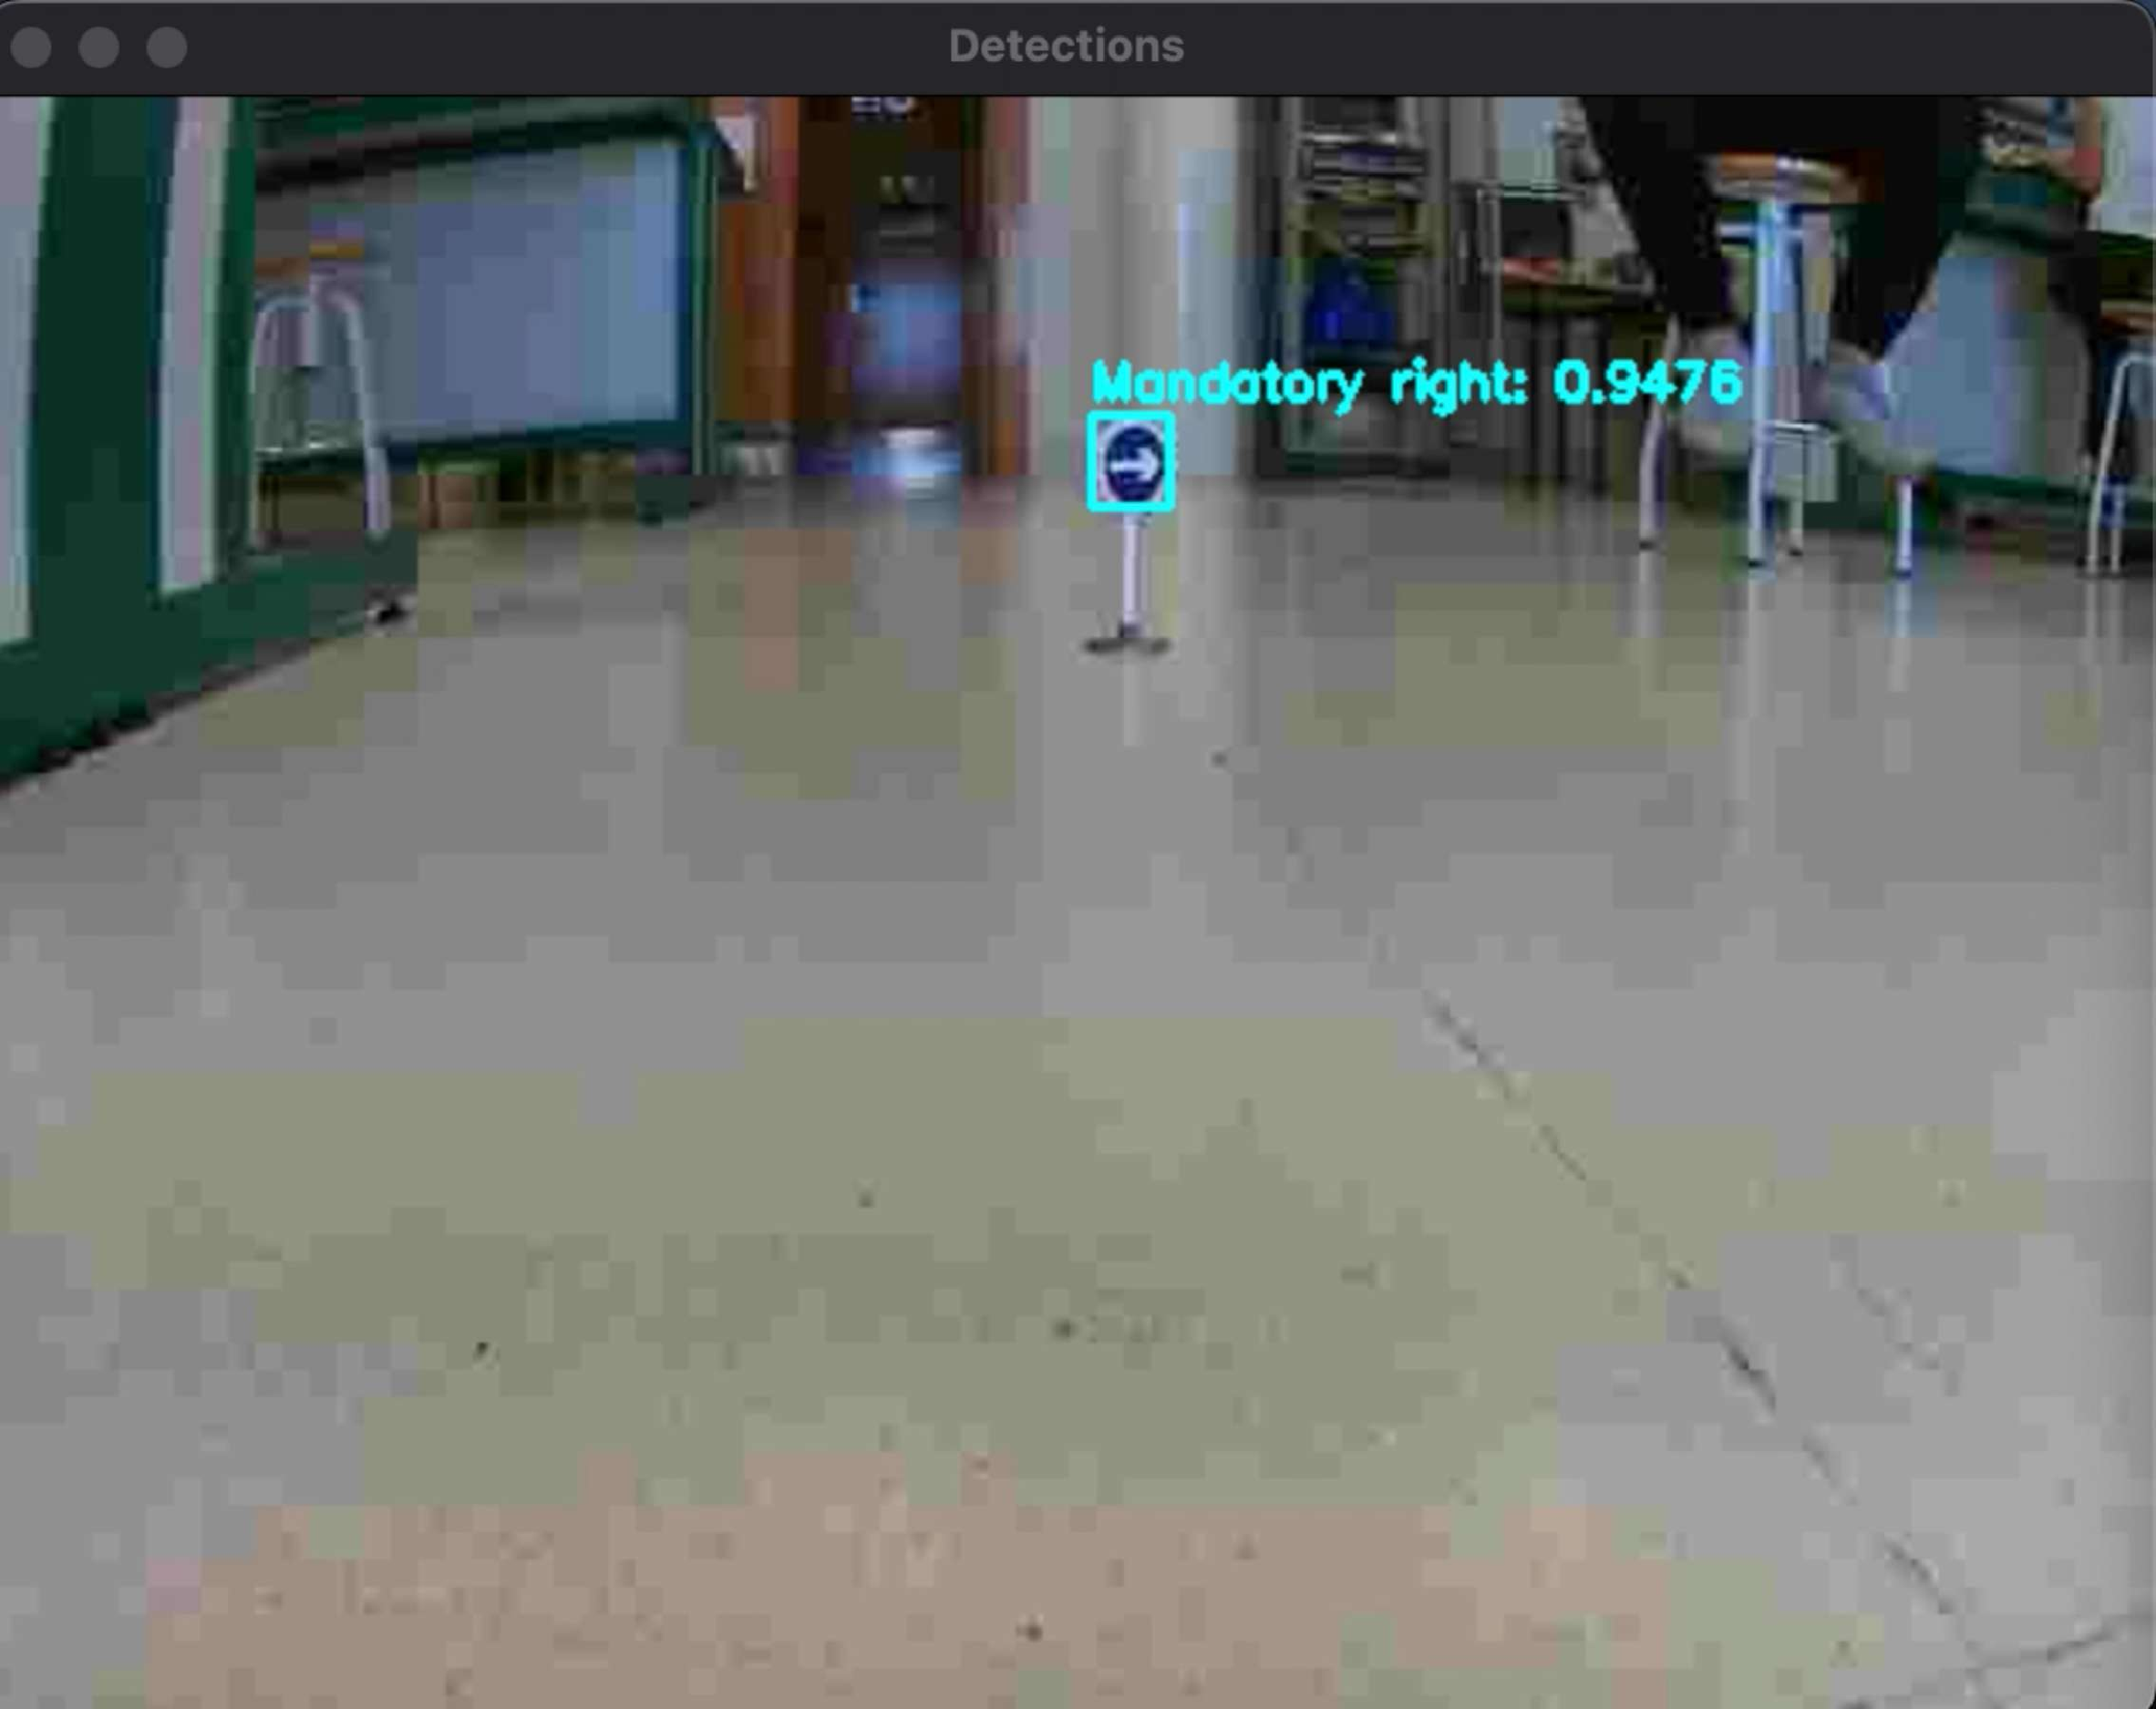
\includegraphics[width=\textwidth]{Imagenes/IA/YoloCNN_coche3.pdf}
    \caption{Resultados de la prueba (4).}
    \label{c4}
\end{figure}

Sin embargo, a pesar de quedar satisfechos con los resultados obtenidos, hemos encontrado ocasiones en las que no detecta bien cada señal, como podemos observar en la señal de limitación 30 km/h \ref{fallo}. \\

\begin{figure}[H]
    \centering
 	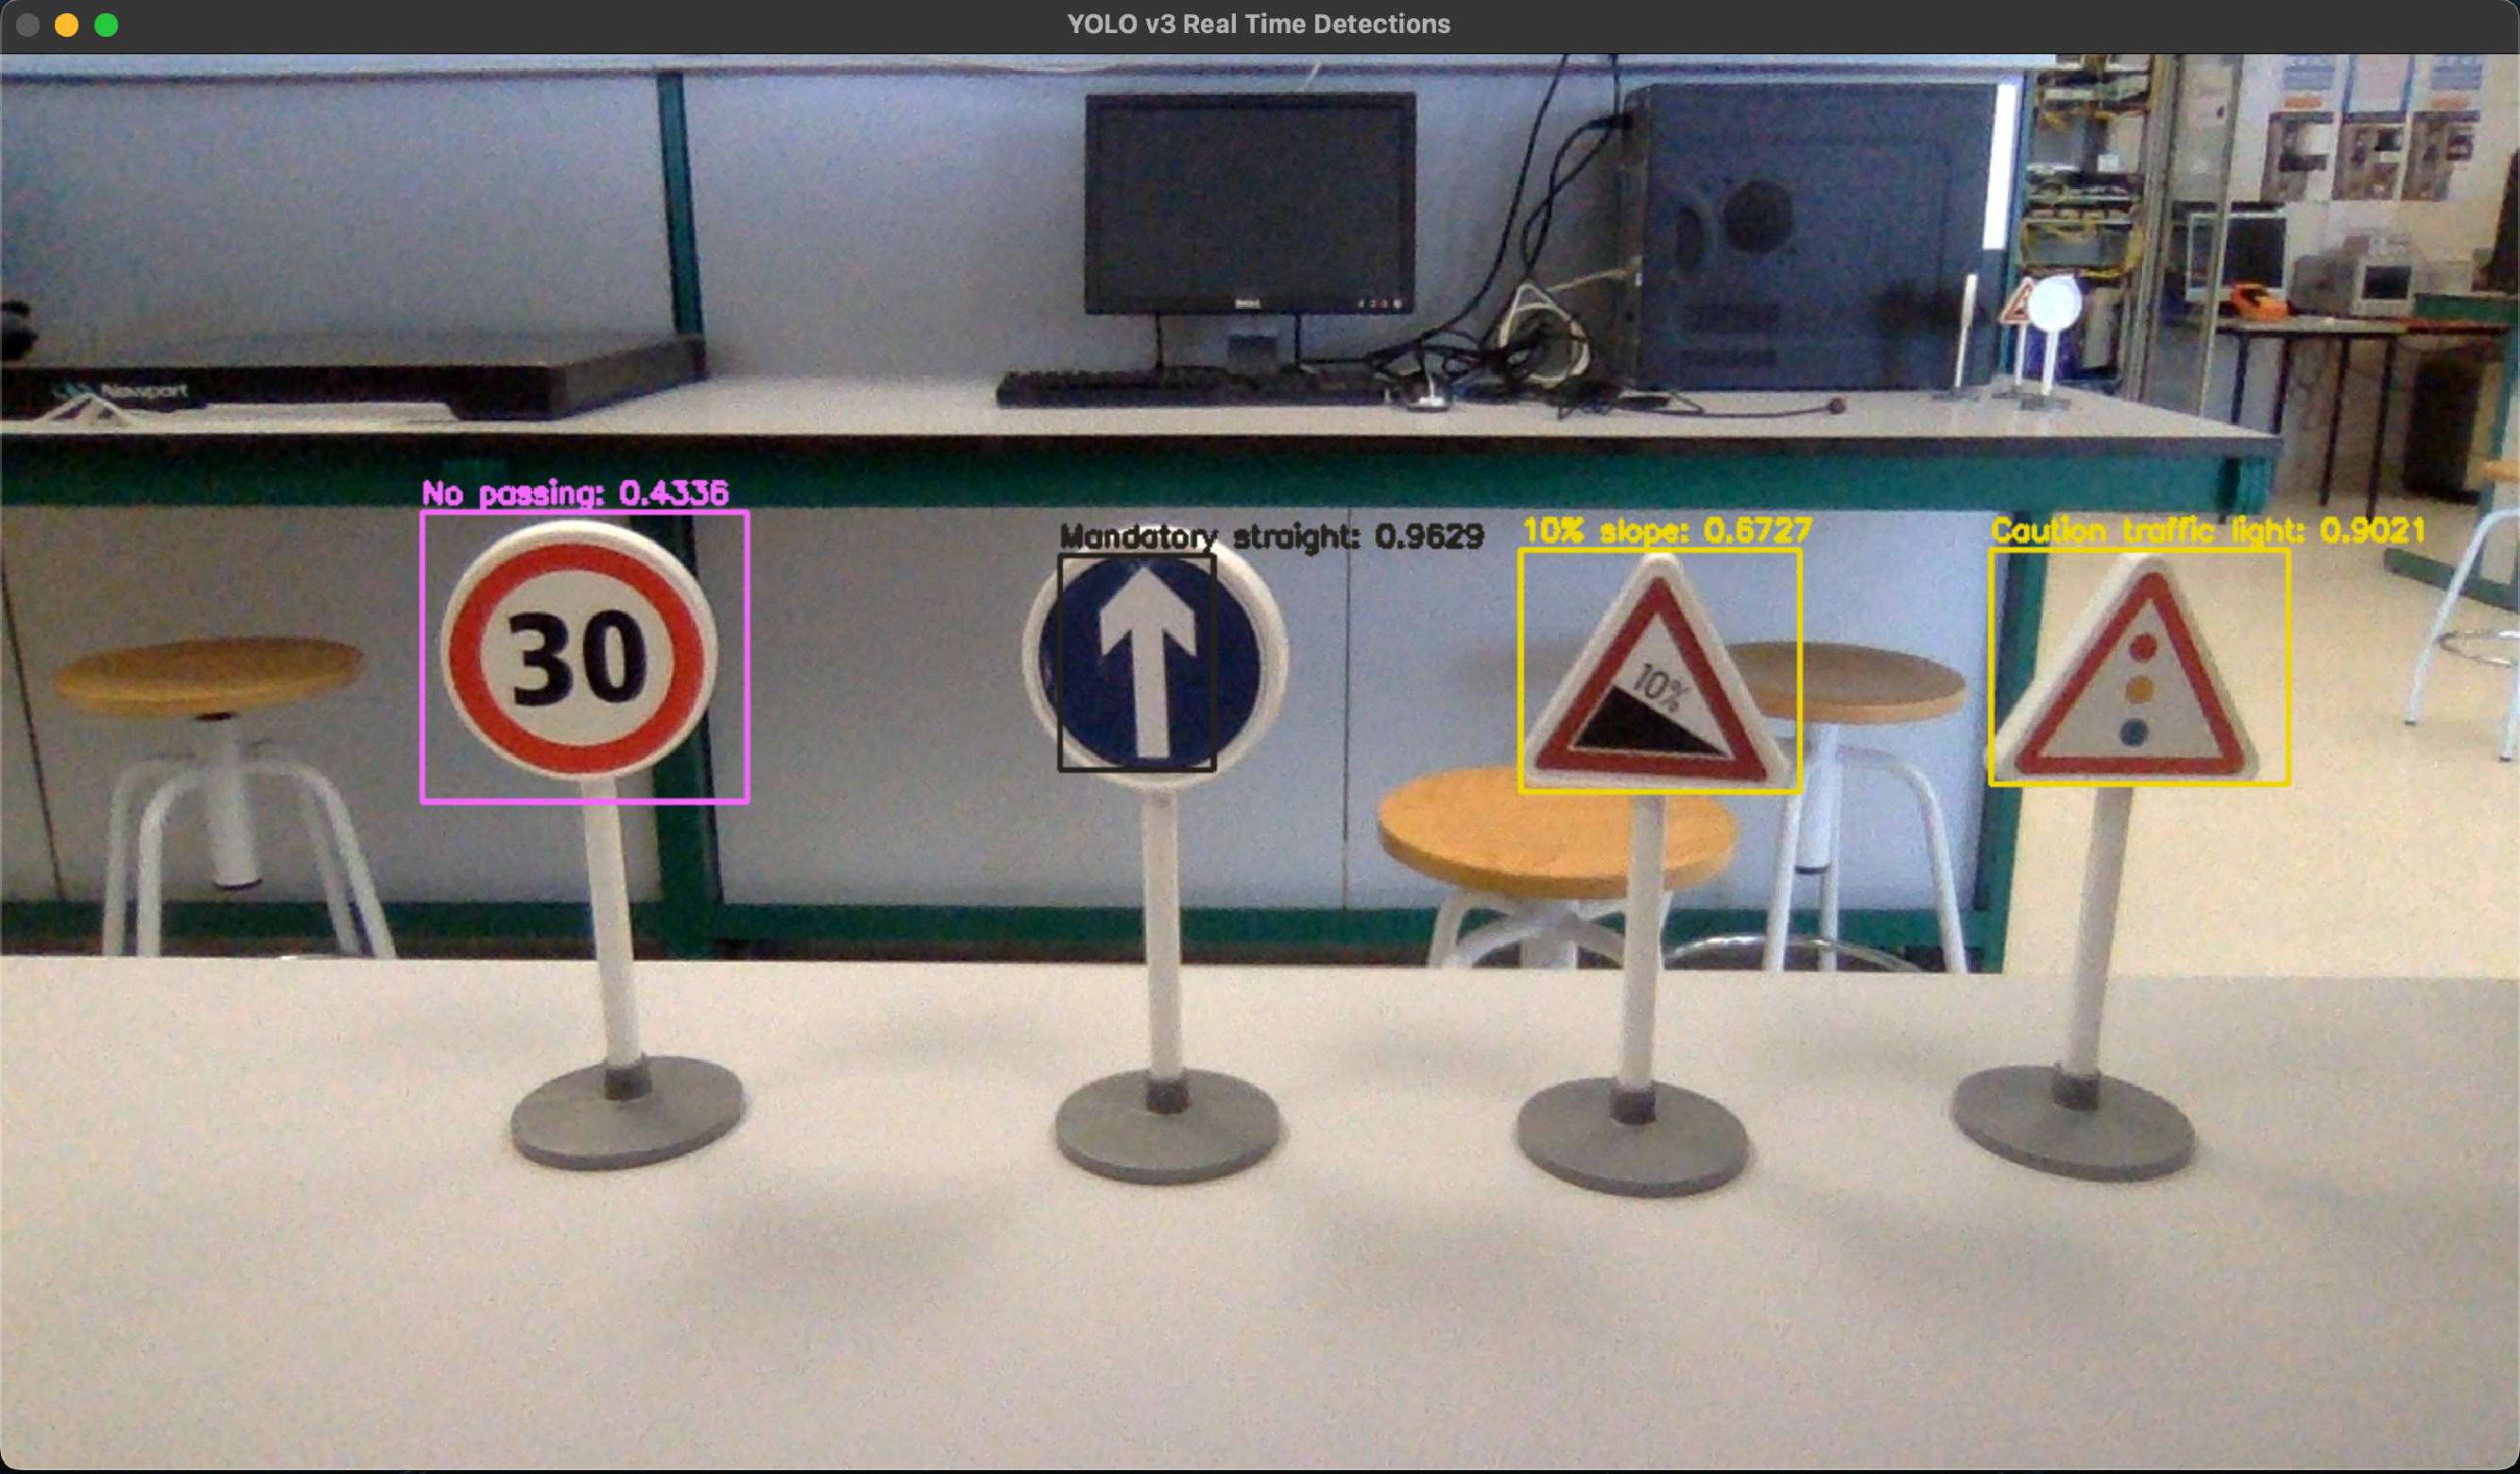
\includegraphics[width=\textwidth]{Imagenes/IA/ejemplo_fallo.pdf}
    \caption{Fallo de detección.}
    \label{fallo}
\end{figure}

Esto puede ser debido a que las condiciones de calidad de imagen que se obtienen de la cámara del propio vehículo no son exactamente las mismas que las imágenes con las que ha sido entrenado. De cara a líneas futuras sería interesante que el conjunto de imágenes creado para el entrenamiento, se diseñara a partir de vídeos grabados por coche.\\

En último lugar, según se puede constatar en el Anexo I apartado 6.2, también hemos utilizado una herramienta de etiquetado denominada LabelIMG \url{https://github.com/heartexlabs/labelImg}. Sería recomendable atender al manual de desarrollador incluido en dicho anexo para aprender a manejar o conocer más detalles acerca del sistema de inteligencia artificial.


